% Presentacion del proyecto final de Calculo Multivariable: Ley de Hooke.
% Compilar desde la carpeta presentacion/ (despues de python regresion_hooke.py):
%   latexmk -pdf presentacion_hooke.tex
\documentclass[aspectratio=169,11pt]{beamer}

\usetheme[progressbar=frametitle,numbering=fraction,sectionpage=none,block=fill]{metropolis}
\usepackage[spanish,es-nodecimaldot,es-noshorthands]{babel}
\usepackage[utf8]{inputenc}
\usepackage[T1]{fontenc}
\usepackage[sfdefault,lining]{FiraSans}
\usepackage[scale=0.85]{FiraMono}
\usepackage[italic]{mathastext}
\usepackage{amsmath,amssymb}
\usepackage{booktabs,array,multicol,tabularx}
\usepackage{tcolorbox}
\usepackage{listings}
\usepackage{appendixnumberbeamer}
\usepackage{colortbl}

\graphicspath{{../figuras/}{../fotos/}{../diagramas/}}
% Generado por regresion_hooke.py: no editar a mano.
\newcommand{\vaCI}{0{,}01514}
\newcommand{\vseA}{0{,}00126}
\newcommand{\vaLo}{0{,}01223}
\newcommand{\vaHi}{0{,}01804}
\newcommand{\vbCI}{-0{,}070}
\newcommand{\vseB}{0{,}256}
\newcommand{\vbLo}{-0{,}661}
\newcommand{\vbHi}{0{,}521}
\newcommand{\vtB}{-0{,}27}
\newcommand{\vtA}{12{,}0}
\newcommand{\vsReg}{0{,}48}
\newcommand{\vtCrit}{2{,}306}
\newcommand{\vkVal}{64{,}7}
\newcommand{\vkLo}{54{,}3}
\newcommand{\vkHi}{80{,}1}
\newcommand{\vuK}{5{,}4}
\newcommand{\vkRango}{25{,}8}
\newcommand{\vjkMin}{57{,}7}
\newcommand{\vjkMax}{66{,}7}
\newcommand{\vjkMinObj}{alicate}
\newcommand{\vjkMaxObj}{tornillo}
\newcommand{\vmcLo}{63{,}7}
\newcommand{\vmcHi}{65{,}9}
\newcommand{\vmcSd}{0{,}56}
\newcommand{\vbandaP}{1{,}17}
\newcommand{\vbandaC}{0{,}37}
\newcommand{\vuLect}{0{,}029}
\newcommand{\vuY}{0{,}05}
\newcommand{\veMaxY}{0{,}15}
\newcommand{\vuX}{0{,}29}
\newcommand{\veMaxX}{0{,}5}
\newcommand{\vuXy}{0{,}0044}
\newcommand{\vrazon}{9}
\newcommand{\vrazonMax}{2{,}9}
\newcommand{\vrmse}{0{,}43}
\newcommand{\vrmseMm}{4{,}3}
\newcommand{\vrmseG}{29}
\newcommand{\vrmseN}{0{,}28}
\newcommand{\vrmseRango}{7{,}7}
\newcommand{\vrmseMedia}{18}
\newcommand{\vrmseRes}{4{,}3}
\newcommand{\vorA}{0{,}01486}
\newcommand{\vorS}{1{,}88}
\newcommand{\vorK}{66{,}0}
\newcommand{\vorRmse}{0{,}43}
\newcommand{\vpAS}{1{,}86}
\newcommand{\vpArmse}{0{,}43}
\newcommand{\vpArr}{0{,}9474}
\newcommand{\vpAra}{0{,}9408}
\newcommand{\vpAaic}{-12{,}8}
\newcommand{\vpAcv}{0{,}58}
\newcommand{\vpAt}{12{,}00}
\newcommand{\vpAtc}{2{,}306}
\newcommand{\vpBS}{1{,}60}
\newcommand{\vpBrmse}{0{,}40}
\newcommand{\vpBrr}{0{,}9549}
\newcommand{\vpBra}{0{,}9420}
\newcommand{\vpBaic}{-12{,}3}
\newcommand{\vpBcv}{0{,}77}
\newcommand{\vpBt}{1{,}08}
\newcommand{\vpBtc}{2{,}365}
\newcommand{\vpBF}{1{,}17}
\newcommand{\vpBFc}{5{,}59}
\newcommand{\vpCS}{1{,}00}
\newcommand{\vpCrmse}{0{,}32}
\newcommand{\vpCrr}{0{,}9717}
\newcommand{\vpCra}{0{,}9575}
\newcommand{\vpCaic}{-15{,}0}
\newcommand{\vpCcv}{0{,}53}
\newcommand{\vpCt}{1{,}88}
\newcommand{\vpCtc}{2{,}447}
\newcommand{\vpCF}{2{,}57}
\newcommand{\vpCFc}{5{,}14}
\newcommand{\vpDS}{1{,}00}
\newcommand{\vpDrmse}{0{,}32}
\newcommand{\vpDrr}{0{,}9717}
\newcommand{\vpDra}{0{,}9491}
\newcommand{\vpDaic}{-13{,}0}
\newcommand{\vpDcv}{4{,}76}
\newcommand{\vpDt}{0{,}08}
\newcommand{\vpDtc}{2{,}571}
\newcommand{\vpDF}{1{,}43}
\newcommand{\vpDFc}{5{,}41}


% ---------- Colores (los mismos de las graficas) ----------
\definecolor{azul}{HTML}{1F4E79}
\definecolor{azulclaro}{HTML}{E8EEF5}
\definecolor{naranja}{HTML}{E07A1F}
\definecolor{verde}{HTML}{2E8B57}
\definecolor{rojo}{HTML}{C0392B}
\definecolor{gris}{HTML}{6B7280}
\definecolor{fondo}{HTML}{FAFAF7}

\setbeamercolor{frametitle}{bg=azul,fg=white}
\setbeamercolor{progress bar}{fg=naranja,bg=azul!40}
\setbeamercolor{title separator}{fg=naranja}
\setbeamercolor{background canvas}{bg=fondo}
\setbeamercolor{normal text}{fg=black!85}
\setbeamercolor{alerted text}{fg=naranja}
\setbeamercolor{example text}{fg=verde}
\setbeamercolor{block title}{bg=azul!15,fg=azul}
\setbeamercolor{block body}{bg=azul!5}
\setbeamercolor{block title alerted}{bg=naranja!20,fg=naranja!70!black}
\setbeamercolor{block body alerted}{bg=naranja!6}
\setbeamercolor{block title example}{bg=verde!18,fg=verde!70!black}
\setbeamercolor{block body example}{bg=verde!5}
\setbeamercolor{itemize item}{fg=naranja}
\setbeamercolor{enumerate item}{fg=azul}
\setbeamertemplate{itemize item}{\small$\blacktriangleright$}
\setbeamerfont{frametitle}{size=\large,series=\bfseries}
\setbeamerfont{caption}{size=\scriptsize}
\setbeamertemplate{caption}{\centering\insertcaption}


% ---------- Cajas y atajos ----------
\newtcolorbox{resultado}[1][]{colback=azulclaro,colframe=azul,boxrule=0.6pt,arc=2mm,
  left=6pt,right=6pt,top=4pt,bottom=4pt,fontupper=\normalsize,before upper=\raggedright,#1}
\newtcolorbox{nota}[1][]{colback=naranja!8,colframe=naranja,boxrule=0.6pt,arc=2mm,
  left=6pt,right=6pt,top=3pt,bottom=3pt,fontupper=\small,before upper=\raggedright,#1}
\newcommand{\dato}[2]{\begin{tabular}{@{}c@{}}{\Large\bfseries\color{azul}#1}\\[-1pt]{\scriptsize\color{gris}#2}\end{tabular}}
\newcommand{\recom}{\tcbox[on line,colback=naranja,colframe=naranja,coltext=white,boxrule=0pt,arc=1.5mm,
  left=3pt,right=3pt,top=1pt,bottom=1pt]{\scriptsize\bfseries Recomendación}}
\newcommand{\foto}[2]{\begin{minipage}[t]{0.155\textwidth}\centering
  \includegraphics[width=\linewidth,height=0.58\textheight,keepaspectratio]{#1}\\[1pt]{\scriptsize #2}\end{minipage}}

\lstset{basicstyle=\ttfamily\fontsize{6.6}{7.4}\selectfont,keywordstyle=\color{azul}\bfseries,commentstyle=\color{gris}\itshape,
  morekeywords={ALGORITMO,LEER,PARA,CADA,HACER,FIN,SI,ENTONCES,SINO,ESCRIBIR,TERMINAR,DIBUJAR,Y},
  morecomment=[l]{//},columns=fullflexible,keepspaces=true,backgroundcolor=\color{white},
  frame=single,rulecolor=\color{azul!30},xleftmargin=4pt,framexleftmargin=4pt,literate={<-}{{$\leftarrow$}}1}

\title{Regresión lineal y optimización mediante funciones de varias variables}
\subtitle{Proyecto final de Cálculo Multivariable: Ley de Hooke}
\author{[Nombres de los integrantes del grupo]}
\institute{Universidad Cooperativa de Colombia, San Juan de Pasto\\Docente: M.Sc. Alejandro Molina}
\date{2026}

\begin{document}

{\setbeamertemplate{footline}{}
\begin{frame}[plain]
  \begin{columns}[c]
    \column{0.66\textwidth}
    {\color{azul}\LARGE\bfseries Regresión lineal y optimización mediante funciones de varias variables\par}
    \vspace{0.6em}
    {\large Proyecto final de Cálculo Multivariable: Ley de Hooke\par}
    \vspace{0.4em}{\color{naranja}\rule{0.9\linewidth}{1.5pt}}\par\vspace{0.6em}
    {\small [Nombres de los integrantes del grupo]\par\vspace{0.5em}
    Universidad Cooperativa de Colombia, San Juan de Pasto\\Docente: M.Sc. Alejandro Molina\\2026\par}
    \column{0.3\textwidth}
    \centering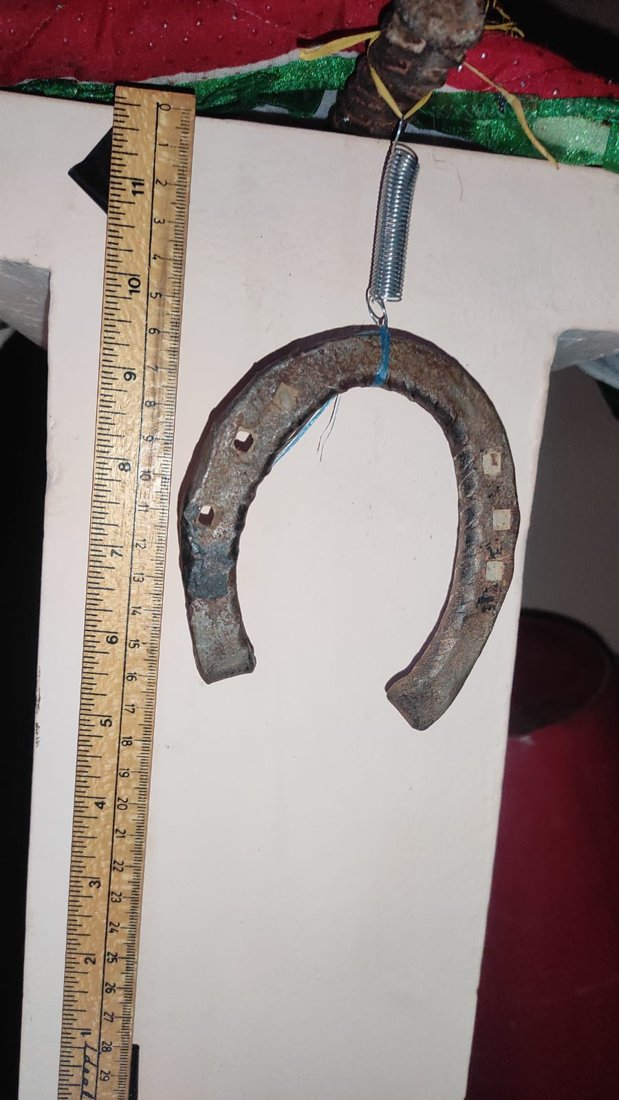
\includegraphics[height=0.86\textheight]{img4.jpg}
  \end{columns}
\end{frame}}

\begin{frame}{Contenido}
  \begin{columns}[T]
    \column{0.48\textwidth}
    \begin{enumerate}\footnotesize\itemsep2pt
      \item Planteamiento del problema
      \item Montaje experimental y datos
      \item Exploración de los datos
      \item Construcción del modelo
      \item Procedimiento analítico
      \item Interpretación geométrica
      \item Verificación computacional
    \end{enumerate}
    \column{0.48\textwidth}
    \begin{enumerate}\footnotesize\itemsep2pt\setcounter{enumi}{7}
      \item Comparación analítico--computacional
      \item Análisis de la recta y de los residuos
      \item Calidad del modelo y RMSE en unidades
      \item \alert{Incertidumbre, sensibilidad y otros modelos}
      \item Influencia de un dato (opción B)
      \item Constante del resorte
      \item Conclusiones y limitaciones
    \end{enumerate}
  \end{columns}
  \vspace{0.4em}
  \begin{nota}[fontupper=\footnotesize]
    \textbf{Nuevo:} errores de la regla y la gramera, intervalos de confianza (valor mínimo y máximo de $k$),
    sensibilidad, regresión polinómica y RMSE en mm, g y N.
  \end{nota}
\end{frame}

% =====================================================================
\section{Planteamiento del problema}

\begin{frame}{1. Introducción y planteamiento del problema}
  \begin{columns}[c]
    \column{0.56\textwidth}
    Al colgar una masa de un resorte, este se estira. La \textbf{Ley de Hooke} dice que, dentro del límite
    elástico, la fuerza es proporcional al estiramiento:
    \[ F = k\,y,\qquad F = m g \;\Rightarrow\; y = \frac{g}{k}\,m . \]
    La teoría predice una relación \textbf{lineal}:
    \[ y = a x + b,\qquad a=\frac{g}{k},\quad b\approx 0 \]
    {\small $x$: masa (g), \quad $y$: estiramiento (cm).}
    \column{0.42\textwidth}
    \begin{block}{Los datos no caen exactamente en una recta}
      Se define el error cuadrático total
      \[ S(a,b)=\sum_{i=1}^{n}\bigl(y_i-a x_i-b\bigr)^2 , \]
      una \textbf{función de dos variables}.
    \end{block}
    \begin{resultado}
      Buscar la mejor recta $=$ buscar el mínimo $(a^*,b^*)$ de $S$.
    \end{resultado}
  \end{columns}
\end{frame}

\begin{frame}{1.1 Pregunta central y objetivo general}
  \begin{resultado}[fontupper=\large\itshape]
    ¿Cómo se puede utilizar el Cálculo Multivariable para determinar y analizar el modelo lineal que mejor
    representa un conjunto de datos?
  \end{resultado}
  \vspace{0.6em}
  \begin{columns}[T]
    \column{0.32\textwidth}
    \begin{block}{Analítica}
      Derivadas parciales, gradiente y Hessiano.
    \end{block}
    \column{0.32\textwidth}
    \begin{block}{Geométrica}
      Superficie, trazas y curvas de nivel.
    \end{block}
    \column{0.32\textwidth}
    \begin{block}{Computacional}
      Programa propio comparado con una biblioteca.
    \end{block}
  \end{columns}
  \vspace{0.6em}
  {\small\textbf{Objetivo general.} Aplicar conceptos de Cálculo Multivariable para formular, resolver y analizar un
  problema de regresión lineal mediante la minimización de una función de error de dos variables, comparando el
  cálculo a mano con el computacional.}
\end{frame}

\begin{frame}{1.2 Objetivos específicos}
  \begin{columns}[T]
    \column{0.49\textwidth}
    \begin{enumerate}\small
      \item Medir el estiramiento del resorte con distintas masas e identificar si la relación es lineal.
      \item Formular la función de error $S(a,b)$.
      \item Calcular a mano las derivadas parciales de $S$.
      \item Usar el gradiente para plantear la condición de punto crítico.
      \item Resolver a mano el sistema y obtener $a^*$ y $b^*$.
    \end{enumerate}
    \column{0.49\textwidth}
    \begin{enumerate}\small\setcounter{enumi}{5}
      \item Calcular el Hessiano y demostrar que el punto crítico es un mínimo.
      \item Programar el procedimiento y compararlo con el cálculo manual y una biblioteca.
      \item Construir gráficas que muestren la minimización.
      \item Analizar la calidad del ajuste, la \textbf{incertidumbre} de los resultados y las limitaciones del
            modelo lineal.
    \end{enumerate}
  \end{columns}
\end{frame}

% =====================================================================
\section{Montaje experimental y datos}

\begin{frame}{2.1 Montaje experimental}
  \begin{columns}[c]
    \column{0.62\textwidth}
    \footnotesize
    Se colgó un resorte de un soporte fijo y, al lado, se fijó una regla de madera. El soporte y la regla no se
    movieron; solo cambió el objeto colgado.
    \begin{itemize}
      \item \textbf{Regla:} resolución de 0,1 cm.
      \item \textbf{Gramera:} masa de cada objeto (resolución 1 g).
    \end{itemize}
    Para cada objeto se midió su masa, su largo y la lectura total del conjunto resorte $+$ objeto:
    \begin{itemize}
      \item Longitud del resorte bajo carga: $L = \text{lectura total} - \text{largo del objeto}$.
      \item Estiramiento: $y = L - L_0$, con $L_0 = 3{,}3$ cm (resorte sin carga).
    \end{itemize}
    El resorte tiene masa propia de 30 g, que no se cuenta como carga: el primer dato es $x=0$ g, $y=0$ cm.
    \column{0.34\textwidth}
    \centering
    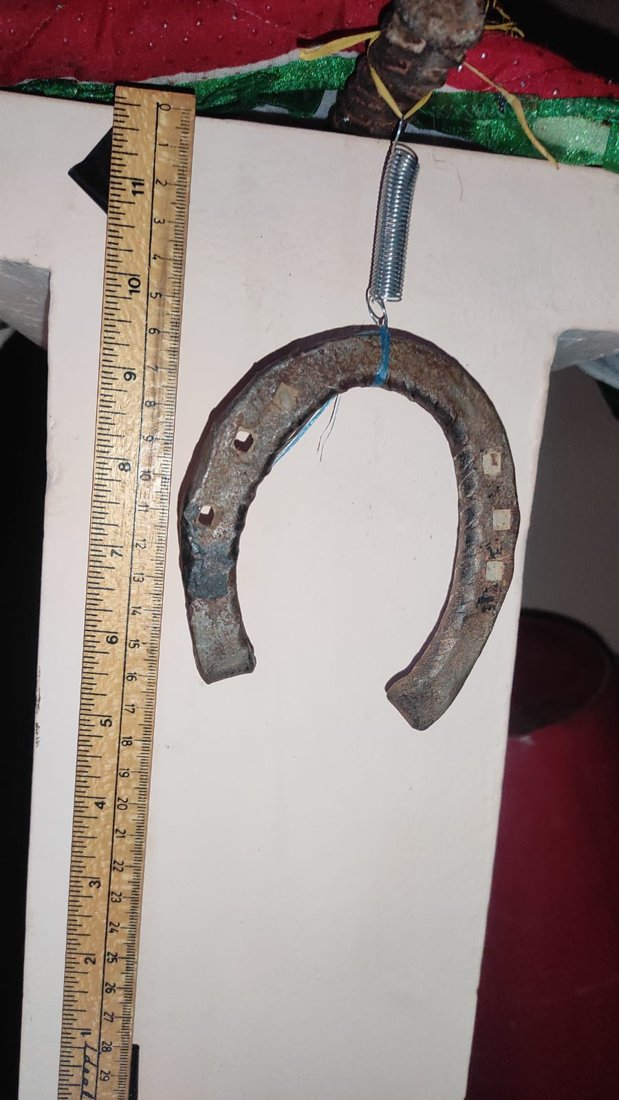
\includegraphics[height=0.7\textheight]{img4.jpg}\\
    {\scriptsize Soporte, resorte y regla (carga: herradura)}
  \end{columns}
\end{frame}

\begin{frame}{2.2 Tabla de datos}
  \centering\small
  \begin{tabular}{rlrrrrr}
    \toprule
    N.º & Objeto colgado & $x$ (g) & Largo obj. (cm) & Lectura total (cm) & $L$ (cm) & $y$ (cm) \\
    \midrule
    1  & Resorte sin carga     & 0   & ---  & 3,3  & 3,3 & 0,0 \\
    2  & Llave grande          & 15  & 7,5  & 10,9 & 3,4 & 0,1 \\
    3  & Tornillo grande       & 70  & 7,1  & 10,8 & 3,7 & 0,4 \\
    4  & Taza plástica         & 92  & 9,5  & 14,4 & 4,9 & 1,6 \\
    5  & Rollo de cinta        & 150 & 11,0 & 16,2 & 5,2 & 1,9 \\
    6  & Herradura             & 185 & 10,9 & 16,7 & 5,8 & 2,5 \\
    7  & Teléfono LG           & 190 & 15,8 & 22,0 & 6,2 & 2,9 \\
    \rowcolor{naranja!12}
    8  & Reproductor / parlante& 220 & 13,1 & 20,6 & 7,5 & 4,2 \\
    9  & Libro pequeño         & 300 & 20,0 & 28,1 & 8,1 & 4,8 \\
    10 & Alicate               & 410 & 22,4 & 31,3 & 8,9 & 5,6 \\
    \bottomrule
  \end{tabular}\\[0.6em]
  {\footnotesize Variable independiente $x$: masa colgada (g). \quad Variable dependiente $y$: estiramiento (cm).}
\end{frame}

\begin{frame}{2.3 Fotografías de las mediciones}
  \centering
  \foto{img3.jpg}{Sin carga}\hfill
  \foto{img5.jpg}{Tornillo grande}\hfill
  \foto{img4.jpg}{Herradura}\hfill
  \foto{img7.jpg}{Teléfono LG}\hfill
  \foto{img2.jpg}{Parlante}\hfill
  \foto{img6.jpg}{Alicate}
  \vfill
  {\footnotesize Fotografías tomadas por el equipo durante el experimento.}
\end{frame}

\begin{frame}{2.3 Las otras cuatro cargas}
  \centering
  \foto{img8.jpg}{Llave grande}\hspace{1.5em}
  \foto{img9.jpg}{Taza plástica}\hspace{1.5em}
  \foto{img10.jpg}{Rollo de cinta}\hspace{1.5em}
  \foto{img11.jpg}{Libro pequeño}
  \vfill
  \begin{nota}
    Imágenes \textbf{ilustrativas}: representan cómo se colgó cada objeto. Los valores de la tabla para estas
    cargas sí fueron medidos por el equipo.
  \end{nota}
\end{frame}

% =====================================================================
\section{Exploración de los datos}

\begin{frame}{3. Exploración de los datos}
  \begin{columns}[c]
    \column{0.6\textwidth}
    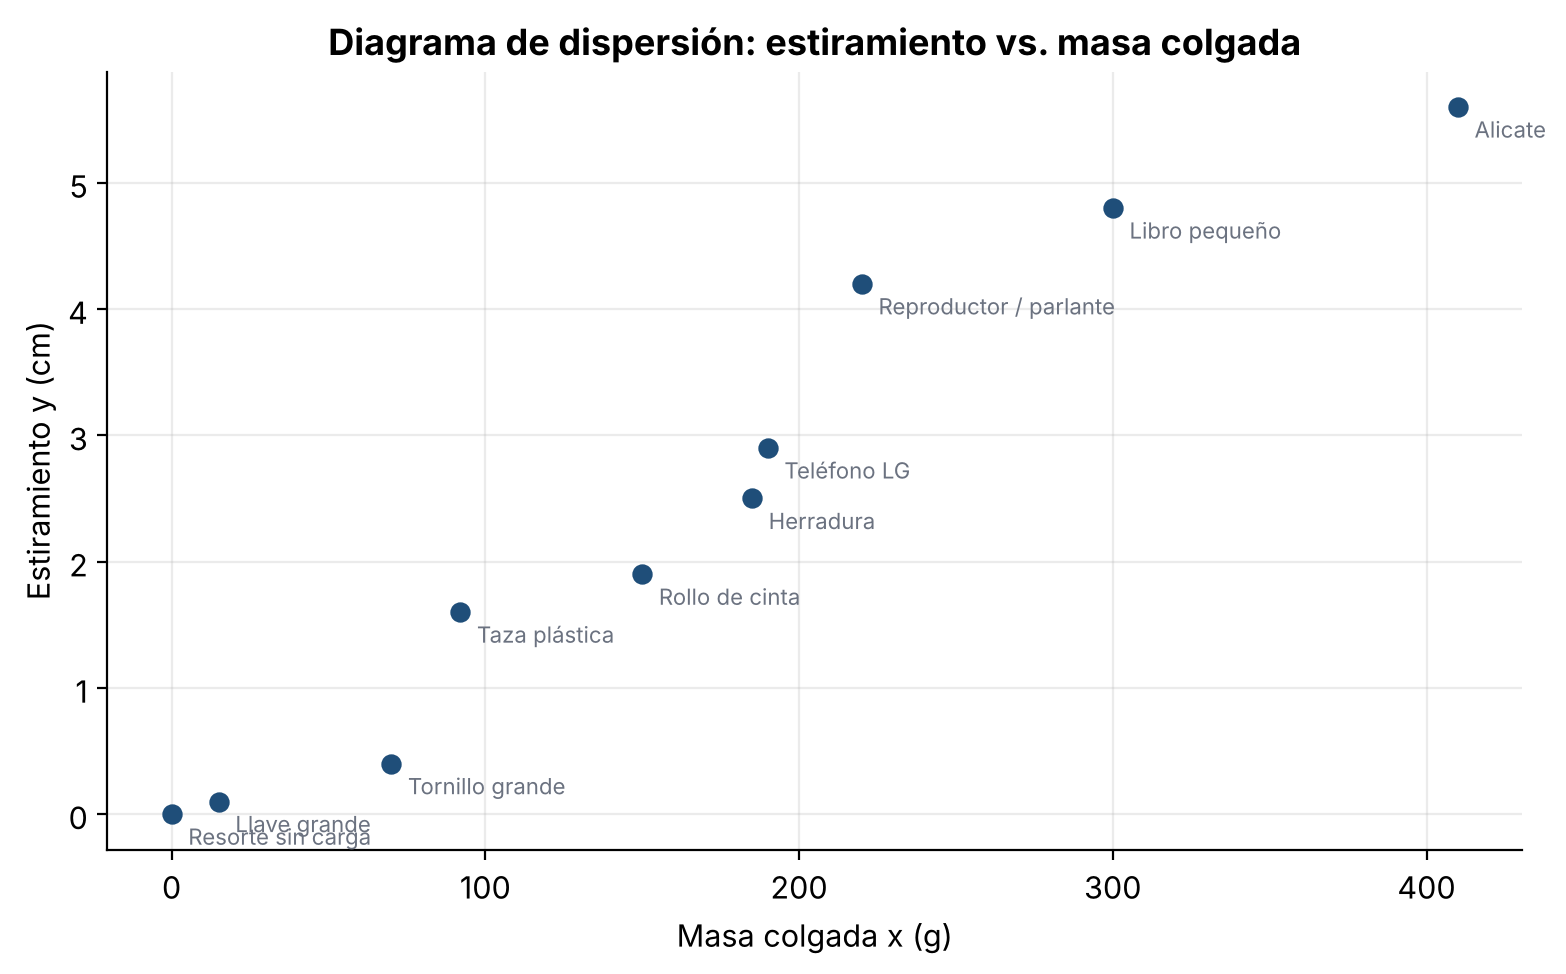
\includegraphics[width=\linewidth]{01_dispersion.png}
    \column{0.38\textwidth}
    \footnotesize
    El estiramiento crece con la masa, sin curvatura clara.
    \begin{resultado}[fontupper=\small]
      $y=ax+b$ es razonable y es el modelo que predice la Ley de Hooke.
    \end{resultado}
    Dos detalles para después:
    \begin{itemize}
      \item con 15 g y 70 g el resorte casi no se estira;
      \item el parlante (220 g) queda por encima de sus vecinos.
    \end{itemize}
  \end{columns}
\end{frame}

\begin{frame}{3.1 Ideas preliminares: ¿por qué una recta?}
  \begin{columns}[T]
    \column{0.49\textwidth}
    \begin{block}{La física lo predice}
      Hooke: $F=ky$ y $F=mg$, luego $y=\frac{g}{k}m$: una recta con pendiente $a=g/k$.
    \end{block}
    \begin{block}{Los datos lo respaldan}
      El diagrama de dispersión no muestra curvatura clara (se comprueba en la sección 11 con polinomios).
    \end{block}
    \column{0.49\textwidth}
    \begin{block}{¿Por qué incluir $b$?}
      Si Hooke se cumple, $b\approx 0$: incluirlo permite \emph{comprobarlo} y hace de $S$ una función de dos
      variables (gradiente y Hessiano).
    \end{block}
    \begin{block}{¿Por qué el error al cuadrado?}
      Evita que se cancelen los signos, se puede derivar y castiga más los errores grandes.
    \end{block}
  \end{columns}
\end{frame}

% =====================================================================
\section{Construcción del modelo}

\begin{frame}{4. Construcción del modelo}
  Modelo lineal $y=ax+b$. Para cada masa $x_i$ el modelo predice $\hat y_i = a x_i + b$, y la diferencia con
  el valor medido es el \textbf{residuo}:
  \[ e_i = y_i - \hat y_i = y_i - (a x_i + b). \]
  Como unos residuos son positivos y otros negativos, se suman sus cuadrados:
  \[ S(a,b)=\sum_{i=1}^{n} e_i^2=\sum_{i=1}^{n}\bigl(y_i-a x_i-b\bigr)^2 . \]
  Los $x_i, y_i$ son números fijos; \textbf{las variables de $S$ son $a$ y $b$}. Con $n=10$:
  \begin{resultado}
    \centering $S(a,b)=412\,914\,a^2+3264\,ab+10\,b^2-12\,270{,}4\,a-48\,b+93{,}04$
  \end{resultado}
\end{frame}

% =====================================================================
\section{Procedimiento analítico}

\begin{frame}{5.1 Derivadas parciales}
  Con la regla de la cadena:
  \begin{align*}
    \frac{\partial S}{\partial a} &= \sum_{i=1}^{n} 2\bigl(y_i-a x_i-b\bigr)(-x_i) = -2\sum_{i=1}^{n} x_i\bigl(y_i-a x_i-b\bigr)\\[4pt]
    \frac{\partial S}{\partial b} &= \sum_{i=1}^{n} 2\bigl(y_i-a x_i-b\bigr)(-1) = -2\sum_{i=1}^{n} \bigl(y_i-a x_i-b\bigr)
  \end{align*}
  \begin{nota}
    Cada dato aporta un término; $\partial S/\partial a$ pesa más los datos con $x_i$ grande.
  \end{nota}
\end{frame}

\begin{frame}{5.1.1 El gradiente: derivadas parciales evaluadas}
  El \textbf{gradiente} agrupa las dos derivadas: $\nabla S=\bigl(\partial S/\partial a,\ \partial S/\partial b\bigr)$.
  Con las sumas de los datos:
  \[ \frac{\partial S}{\partial a}=-2\sum x_iy_i+2a\sum x_i^2+2b\sum x_i, \qquad
     \frac{\partial S}{\partial b}=-2\sum y_i+2a\sum x_i+2nb \]
  \begin{columns}[c]
    \column{0.55\textwidth}
    Evaluado en la recta A $(a=0,\ b=0)$:
    \[ \frac{\partial S}{\partial a}=-12\,270{,}4,\quad \frac{\partial S}{\partial b}=-48,\quad S=93{,}04 \]
    \column{0.42\textwidth}
    \begin{resultado}[fontupper=\small]
      Ambos signos son negativos: el error \textbf{baja} si se aumentan $a$ y $b$.
    \end{resultado}
  \end{columns}
\end{frame}

\begin{frame}{5.1.2 Una suma de aportes da un solo valor}
  \centering
  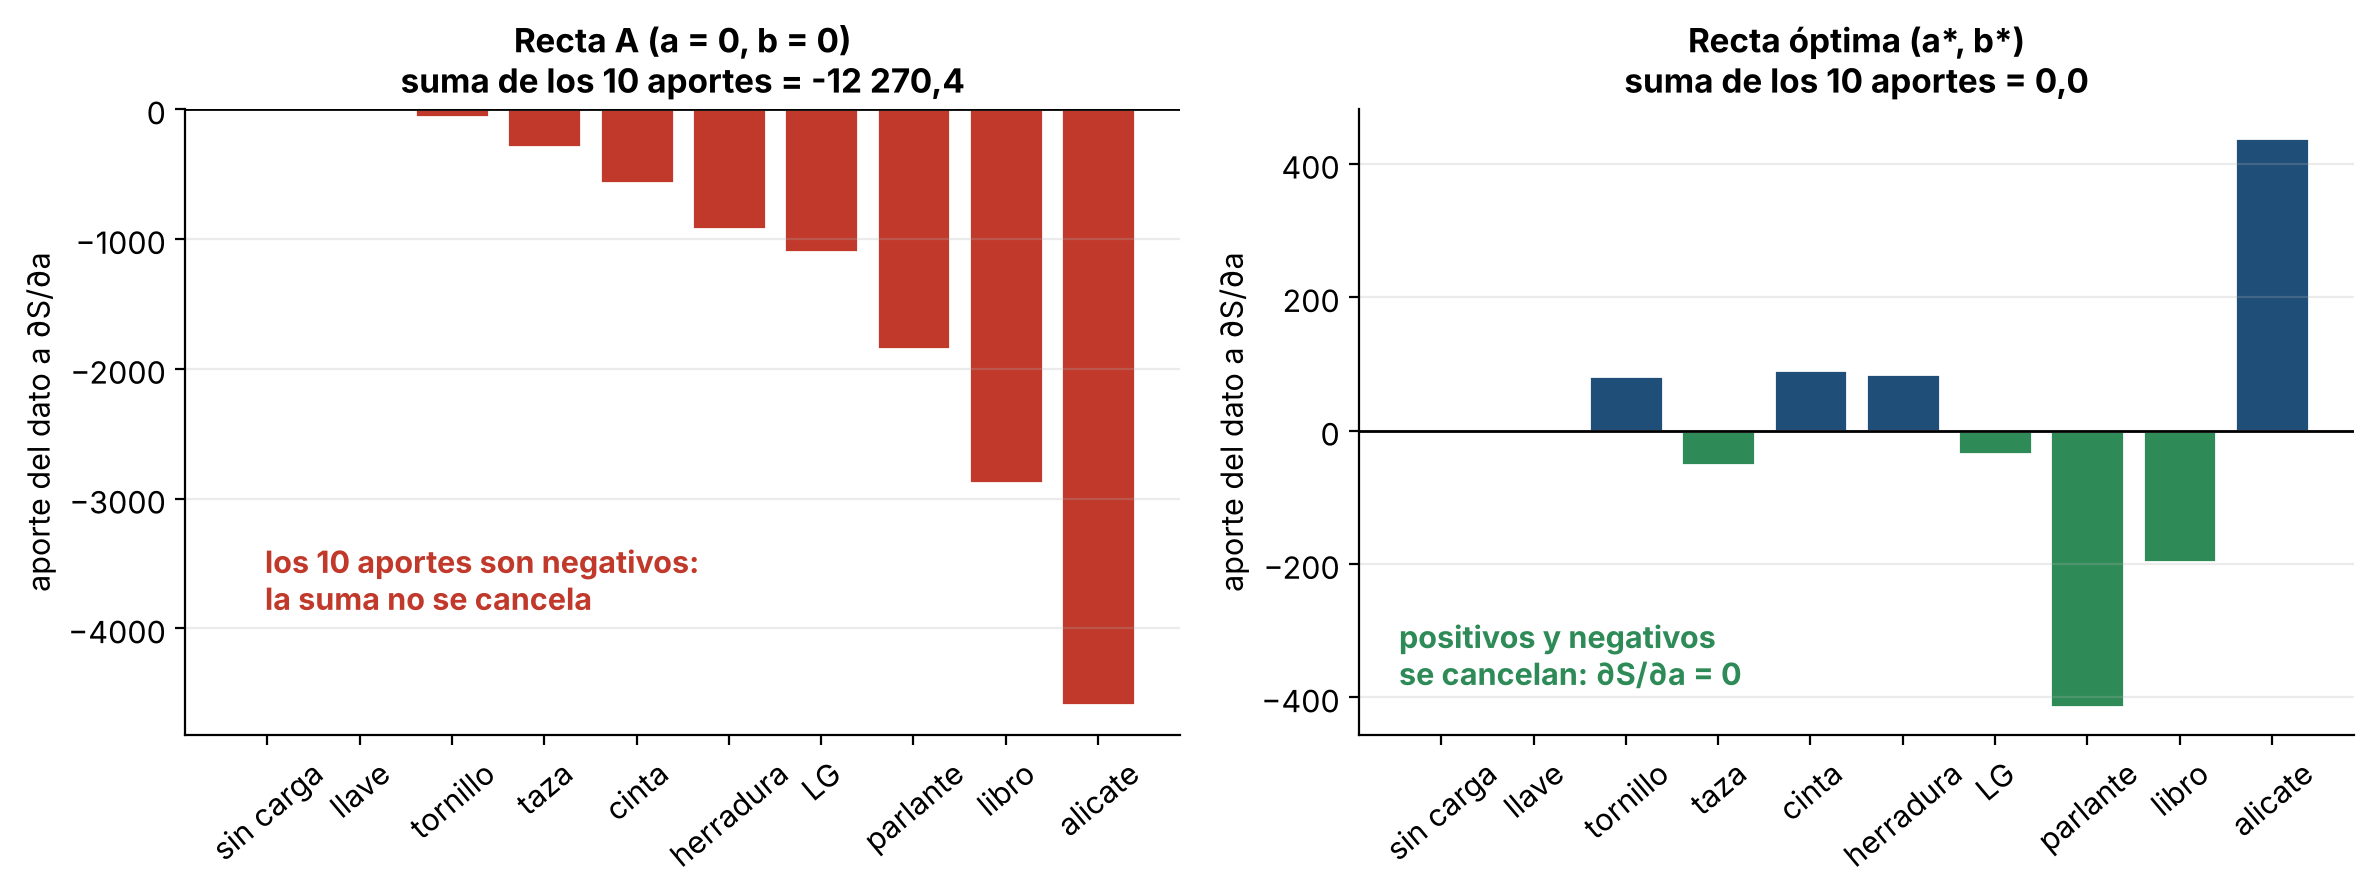
\includegraphics[width=0.95\linewidth]{09_aportes_gradiente.png}\par\vspace{0.3em}
  {\small Cada dato ``jala'' la recta; la derivada es el jalón total. En el óptimo los jalones se equilibran.}
\end{frame}

\begin{frame}{5.2 Condición de punto crítico}
  El punto crítico cumple $\nabla S(a,b)=(0,0)$. Al dividir entre $-2$ y separar las sumas se obtienen las
  \textbf{ecuaciones normales}:
  \begin{resultado}
    \[ \begin{cases} a\sum x_i^2 + b\sum x_i = \sum x_iy_i\\[3pt] a\sum x_i + n\,b = \sum y_i \end{cases} \]
  \end{resultado}
  Es un sistema lineal $2\times 2$ en las incógnitas $a$ y $b$.
\end{frame}

\begin{frame}{5.3 Determinación de los parámetros}
  \small Sumas: $n=10,\ \sum x_i=1632,\ \sum y_i=24,\ \sum x_i^2=412\,914,\ \sum x_iy_i=6135{,}2$.
  \[ \begin{cases} 412\,914\,a+1632\,b=6135{,}2\\ 1632\,a+10\,b=24 \end{cases} \]
  \[ a^*=\frac{n\sum x_iy_i-\sum x_i\sum y_i}{n\sum x_i^2-\left(\sum x_i\right)^2}
       =\frac{61\,352-39\,168}{4\,129\,140-2\,663\,424}=\frac{22\,184}{1\,465\,716}=0{,}0151353\ \text{cm/g} \]
  \[ b^*=\frac{\sum y_i-a^*\sum x_i}{n}=\frac{24-24{,}7008096}{10}=-0{,}0700810\ \text{cm} \]
  \begin{resultado}
    \centering\textbf{Recta de mejor ajuste:}\quad $y=0{,}0151\,x-0{,}070$ \quad ($x$ en g, $y$ en cm),
    \quad $S(a^*,b^*)=1{,}8639\ \text{cm}^2$
  \end{resultado}
\end{frame}

\begin{frame}{5.4 Análisis mediante el Hessiano}
  Las segundas derivadas son constantes:
  \[ S_{aa}=2\sum x_i^2=825\,828,\qquad S_{bb}=2n=20,\qquad S_{ab}=S_{ba}=2\sum x_i=3264 . \]
  \[ H=\begin{pmatrix}825\,828 & 3264\\ 3264 & 20\end{pmatrix},\qquad \det H=825\,828\cdot 20-3264^2=5\,862\,864 . \]
  \begin{columns}[T]
    \column{0.42\textwidth}
    \begin{resultado}[fontupper=\small]
      $\det H>0$ y $S_{aa}>0$: $(a^*,b^*)$ es un \textbf{mínimo}. Como $H$ es constante y definida positiva,
      $S$ es convexa: el mínimo es \textbf{único y global}.
    \end{resultado}
    \column{0.55\textwidth}
    \small En general
    \[ \det H=4\Bigl[n\sum x_i^2-\bigl(\textstyle\sum x_i\bigr)^2\Bigr]=4n\sum(x_i-\bar x)^2>0 \]
    si hay al menos dos masas distintas.
  \end{columns}
\end{frame}

\begin{frame}{5.5 Preguntas clave: gradiente, mínimo y silla de montar}
  \small
  \begin{columns}[T]
    \column{0.5\textwidth}
    \textbf{¿Qué es el gradiente?} $\nabla S$ apunta hacia donde $S$ \emph{crece} más rápido; $-\nabla S$ hacia
    donde \emph{baja} más rápido. En el mínimo $\nabla S=(0,0)$.

    \medskip
    \textbf{¿Por qué el determinante decide?} $D=\lambda_1\lambda_2$. Si $D<0$, un valor propio es positivo y otro
    negativo: $S$ sube en una dirección y baja en otra (silla).
    \column{0.46\textwidth}
    Con $D=\det H=S_{aa}S_{bb}-S_{ab}^2$:\\[4pt]
    \begin{tabular}{ll}
      \toprule
      Condición & Tipo de punto \\
      \midrule
      $D>0$ y $S_{aa}>0$ & \textcolor{verde}{\textbf{mínimo}} \\
      $D>0$ y $S_{aa}<0$ & máximo \\
      $D<0$ & silla de montar \\
      $D=0$ & no concluye \\
      \bottomrule
    \end{tabular}
  \end{columns}
  \vfill
  \begin{resultado}[fontupper=\small]
    En este proyecto $S_{aa}=2\sum x_i^2>0$ y $D=4n\sum(x_i-\bar x)^2=5\,862\,864>0$: es un mínimo global y
    nunca puede salir silla.
  \end{resultado}
\end{frame}

% =====================================================================
\section{Interpretación geométrica}

\begin{frame}{6.1 Superficie de error}
  \begin{columns}[c]
    \column{0.55\textwidth}
    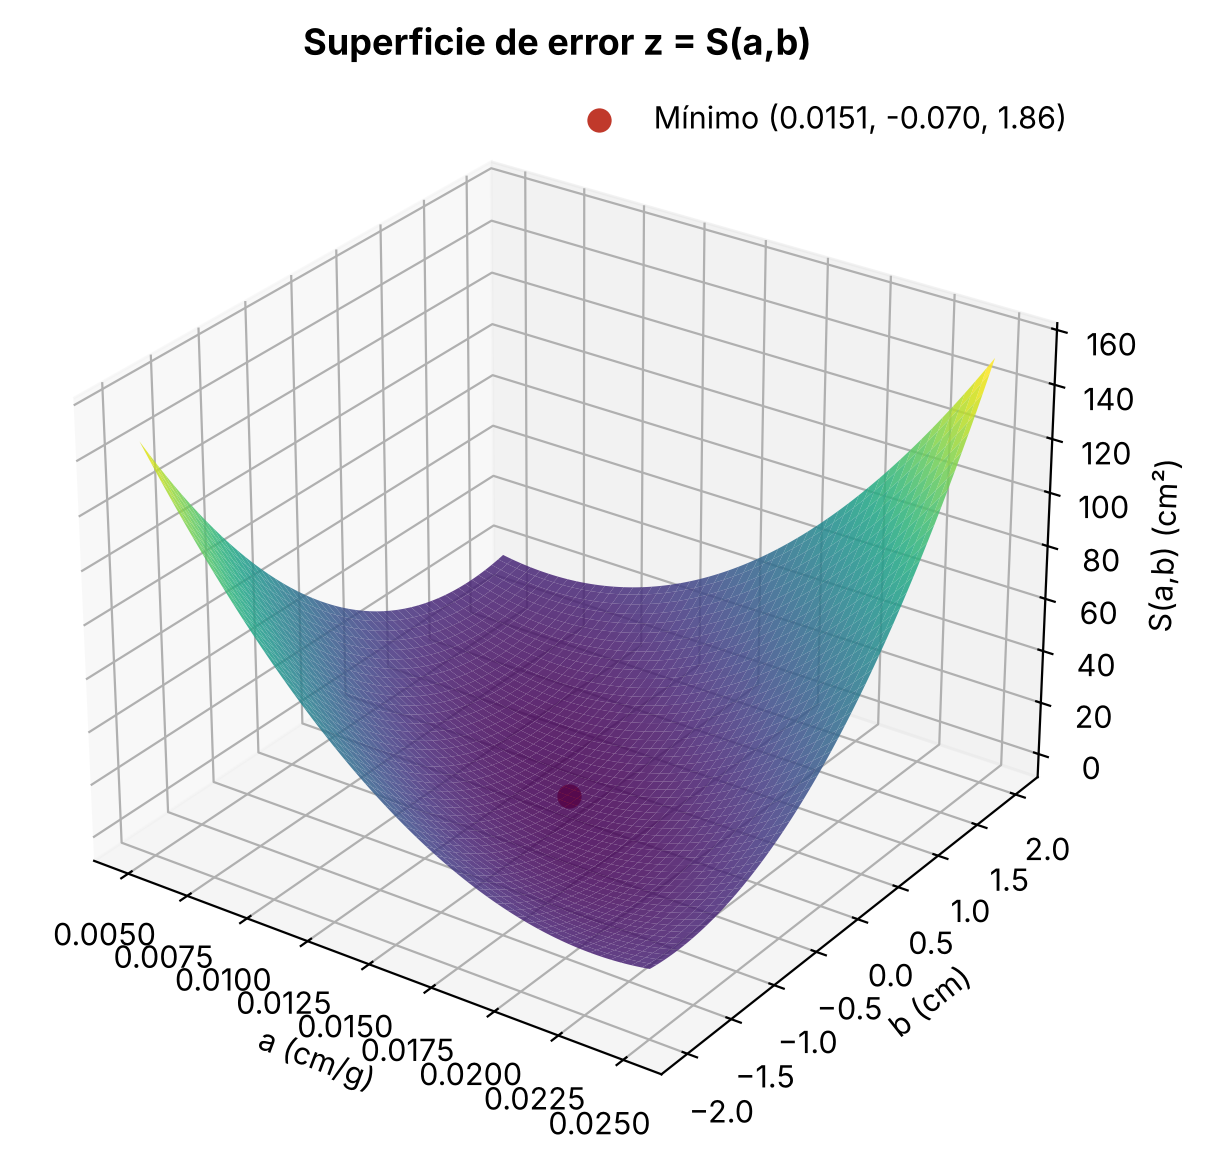
\includegraphics[width=\linewidth]{03_superficie.png}
    \column{0.43\textwidth}
    $z=S(a,b)$ es un \textbf{paraboloide elíptico} que abre hacia arriba, con forma de valle.
    \medskip

    {\small Se graficó para $0{,}005\le a\le 0{,}025$ y $-2\le b\le 2$, un intervalo que contiene al mínimo.}
    \begin{resultado}[fontupper=\small]
      Punto más bajo: $(a^*,b^*)=(0{,}0151;\,-0{,}070)$, con $S=1{,}86$ cm$^2$. En cualquier dirección el error sube.
    \end{resultado}
  \end{columns}
\end{frame}

\begin{frame}{6.2 Trazas y secciones transversales}
  \centering
  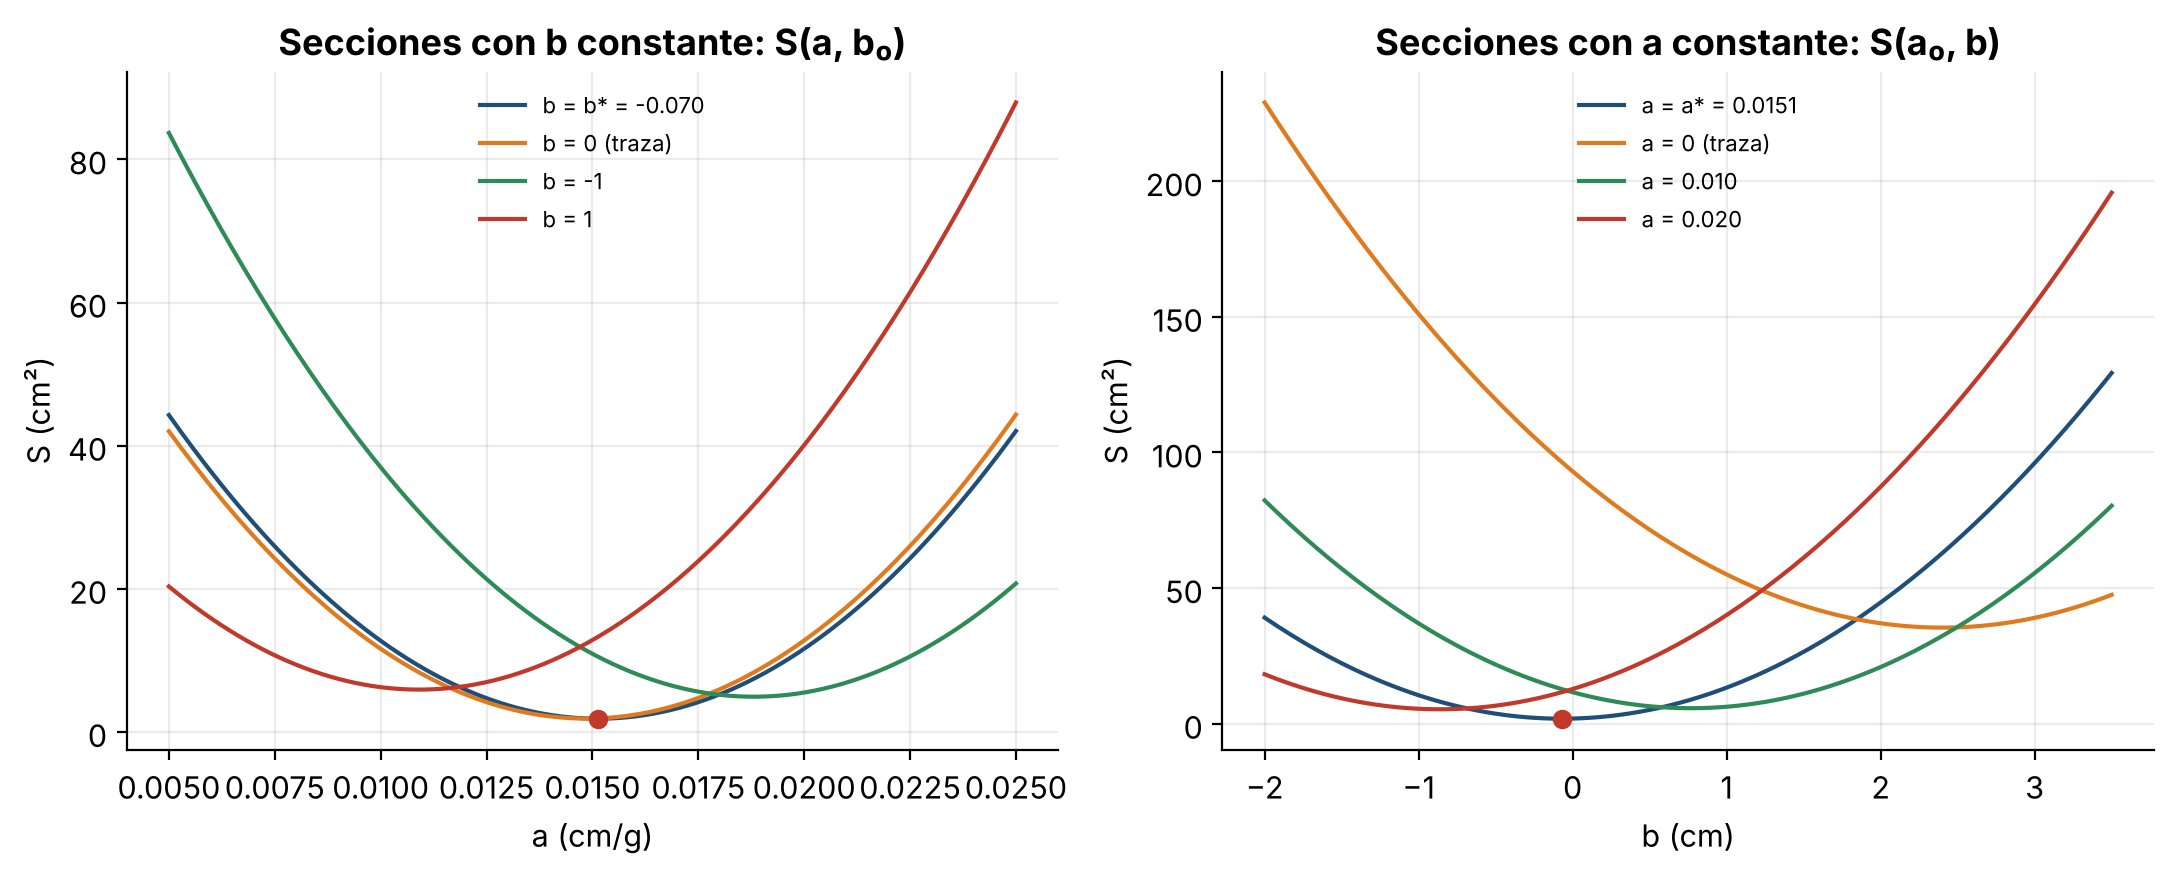
\includegraphics[width=0.92\linewidth]{04_trazas.png}\\[0.2em]
  \begin{columns}[T]
    \column{0.48\textwidth}\footnotesize
    \textbf{$b$ fijo:} cada $S(a,b_0)$ es una parábola. Con $b=0$: $S(a,0)=412\,914a^2-12\,270{,}4a+93{,}04$,
    vértice en $a=0{,}01486$.
    \column{0.48\textwidth}\footnotesize
    \textbf{$a$ fijo:} con $a=0$: $S(0,b)=10b^2-48b+93{,}04$, vértice en $b=2{,}4=\bar y$ y error 35,44
    (mucho mayor que 1,86).
  \end{columns}
\end{frame}

\begin{frame}{6.2 Qué muestran las secciones}
  \begin{itemize}
    \item Todas son parábolas hacia arriba: $S$ tiene un solo mínimo.
    \item El vértice de cada sección se desplaza al cambiar el valor fijo: el mejor $a$ depende del $b$
          escogido y viceversa.
    \item Por eso \textbf{no se pueden optimizar $a$ y $b$ por separado}: hace falta resolver el sistema de
          dos ecuaciones.
    \item La sección con $b=b^*$ es la única que baja hasta el mínimo global.
  \end{itemize}
\end{frame}

\begin{frame}{6.3 Curvas de nivel}
  \begin{columns}[c]
    \column{0.58\textwidth}
    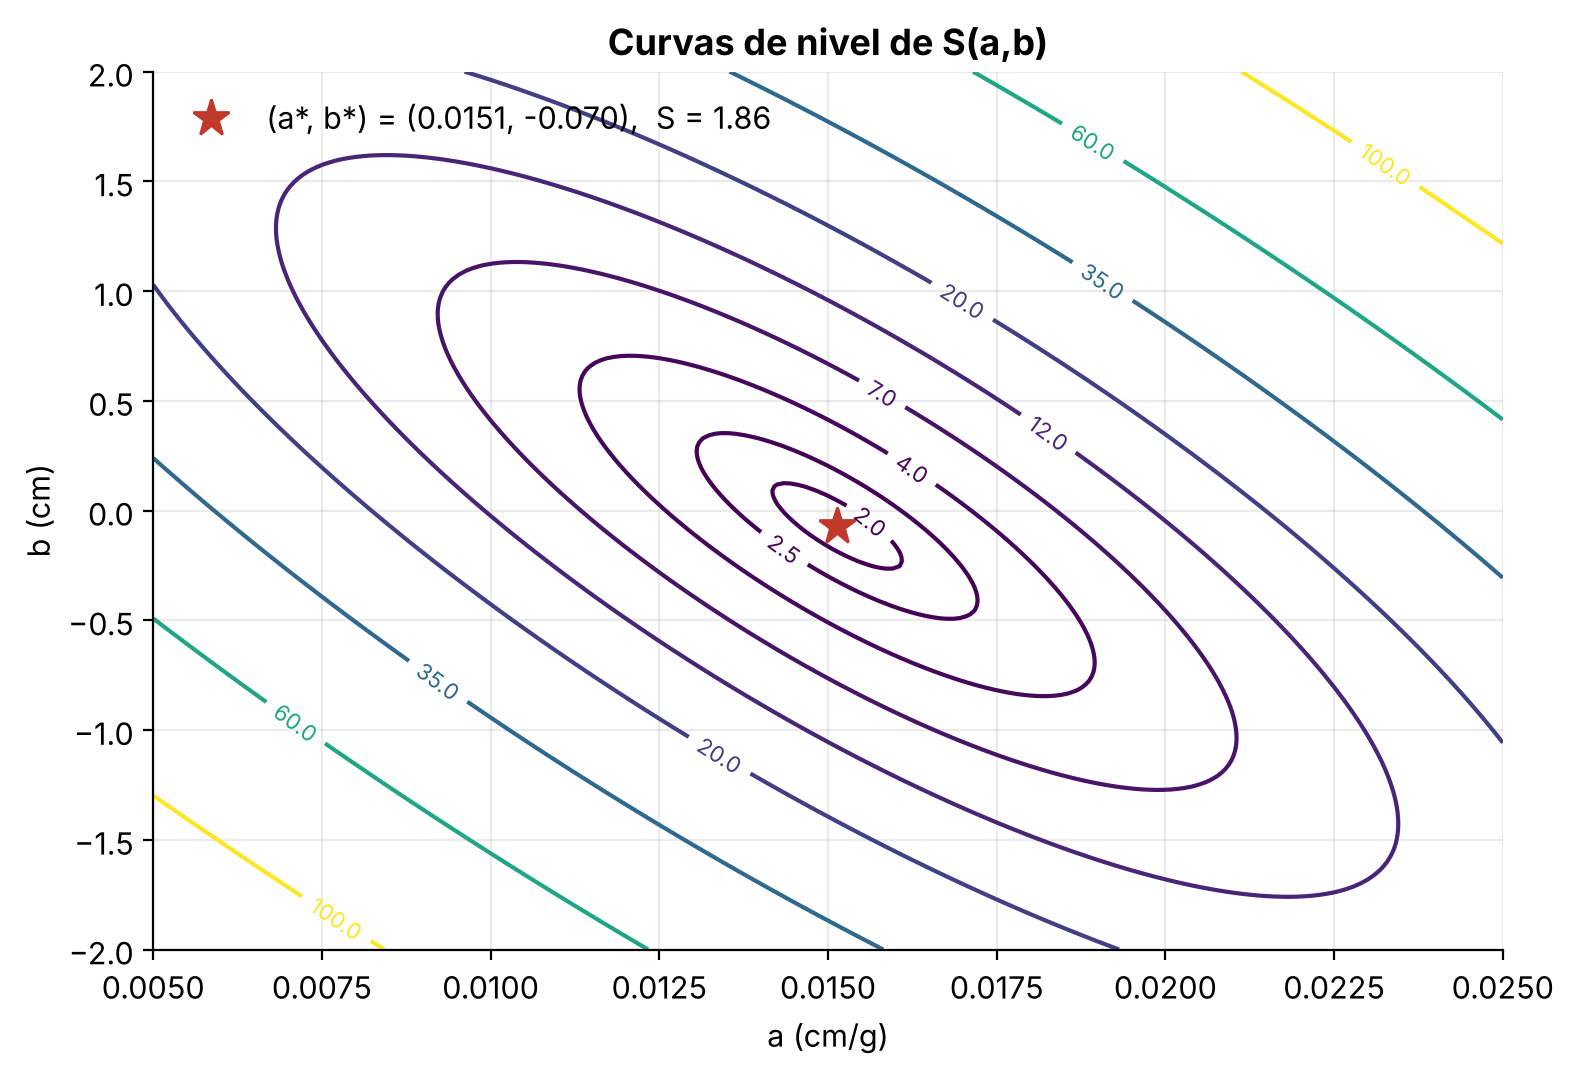
\includegraphics[width=\linewidth]{05_curvas_nivel.png}
    \column{0.4\textwidth}\small
    Cada curva reúne las parejas $(a,b)$ que dan el mismo error. Son \textbf{elipses concéntricas} con centro
    en $(a^*,b^*)$.
    \medskip

    Están inclinadas hacia abajo a la derecha: \textbf{$a$ y $b$ se compensan}. La inclinación viene del
    término cruzado $3264\,ab$, es decir, de $S_{ab}\neq 0$.
  \end{columns}
\end{frame}

\begin{frame}{6.3.1 El gradiente sobre el mapa}
  \centering
  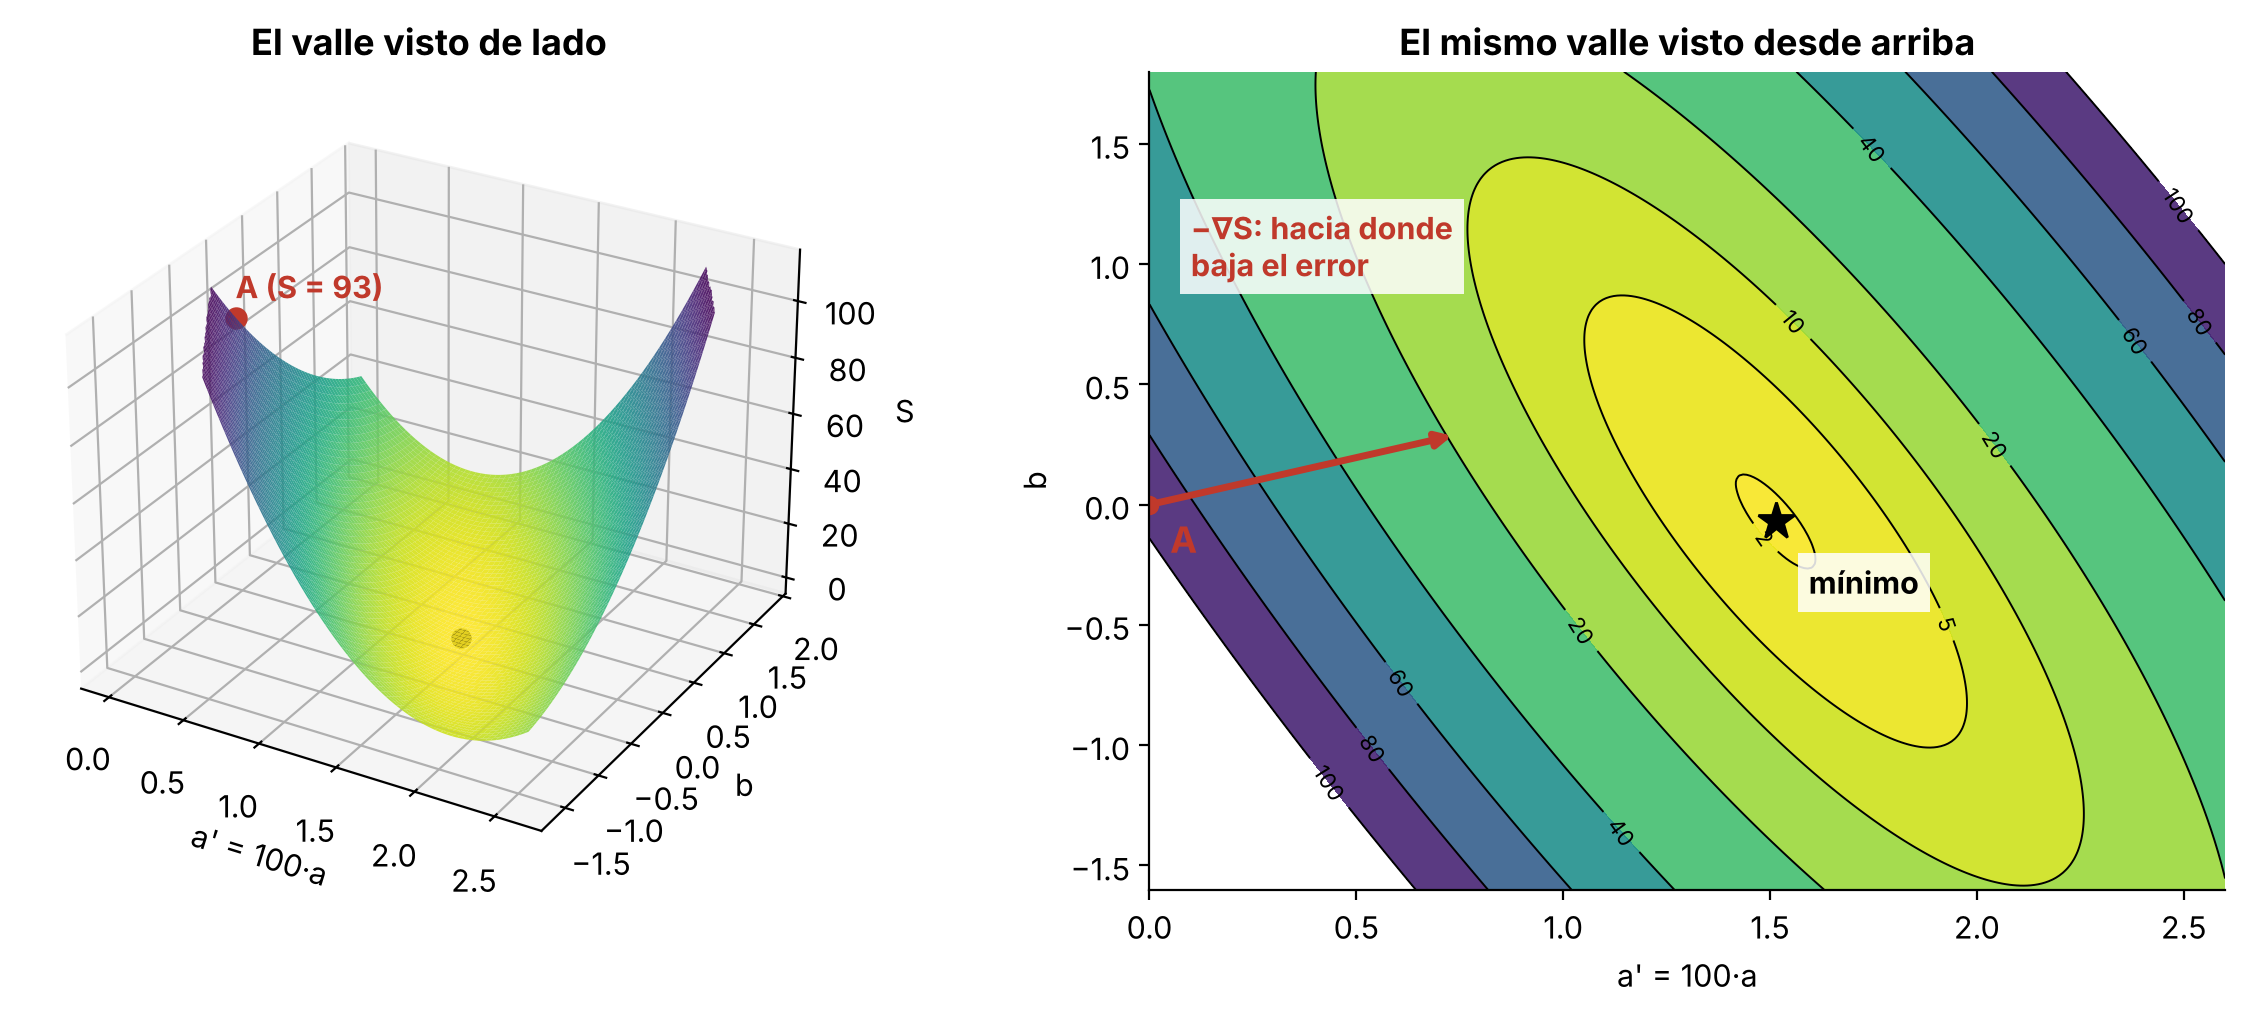
\includegraphics[width=0.92\linewidth]{10_gradiente_mapa.png}\\
  {\small Las curvas de nivel son el mapa topográfico del valle: cada línea es una altura (un valor de $S$).}
\end{frame}

\begin{frame}{6.3.2 El gradiente como vector y el tamaño del paso}
  \centering
  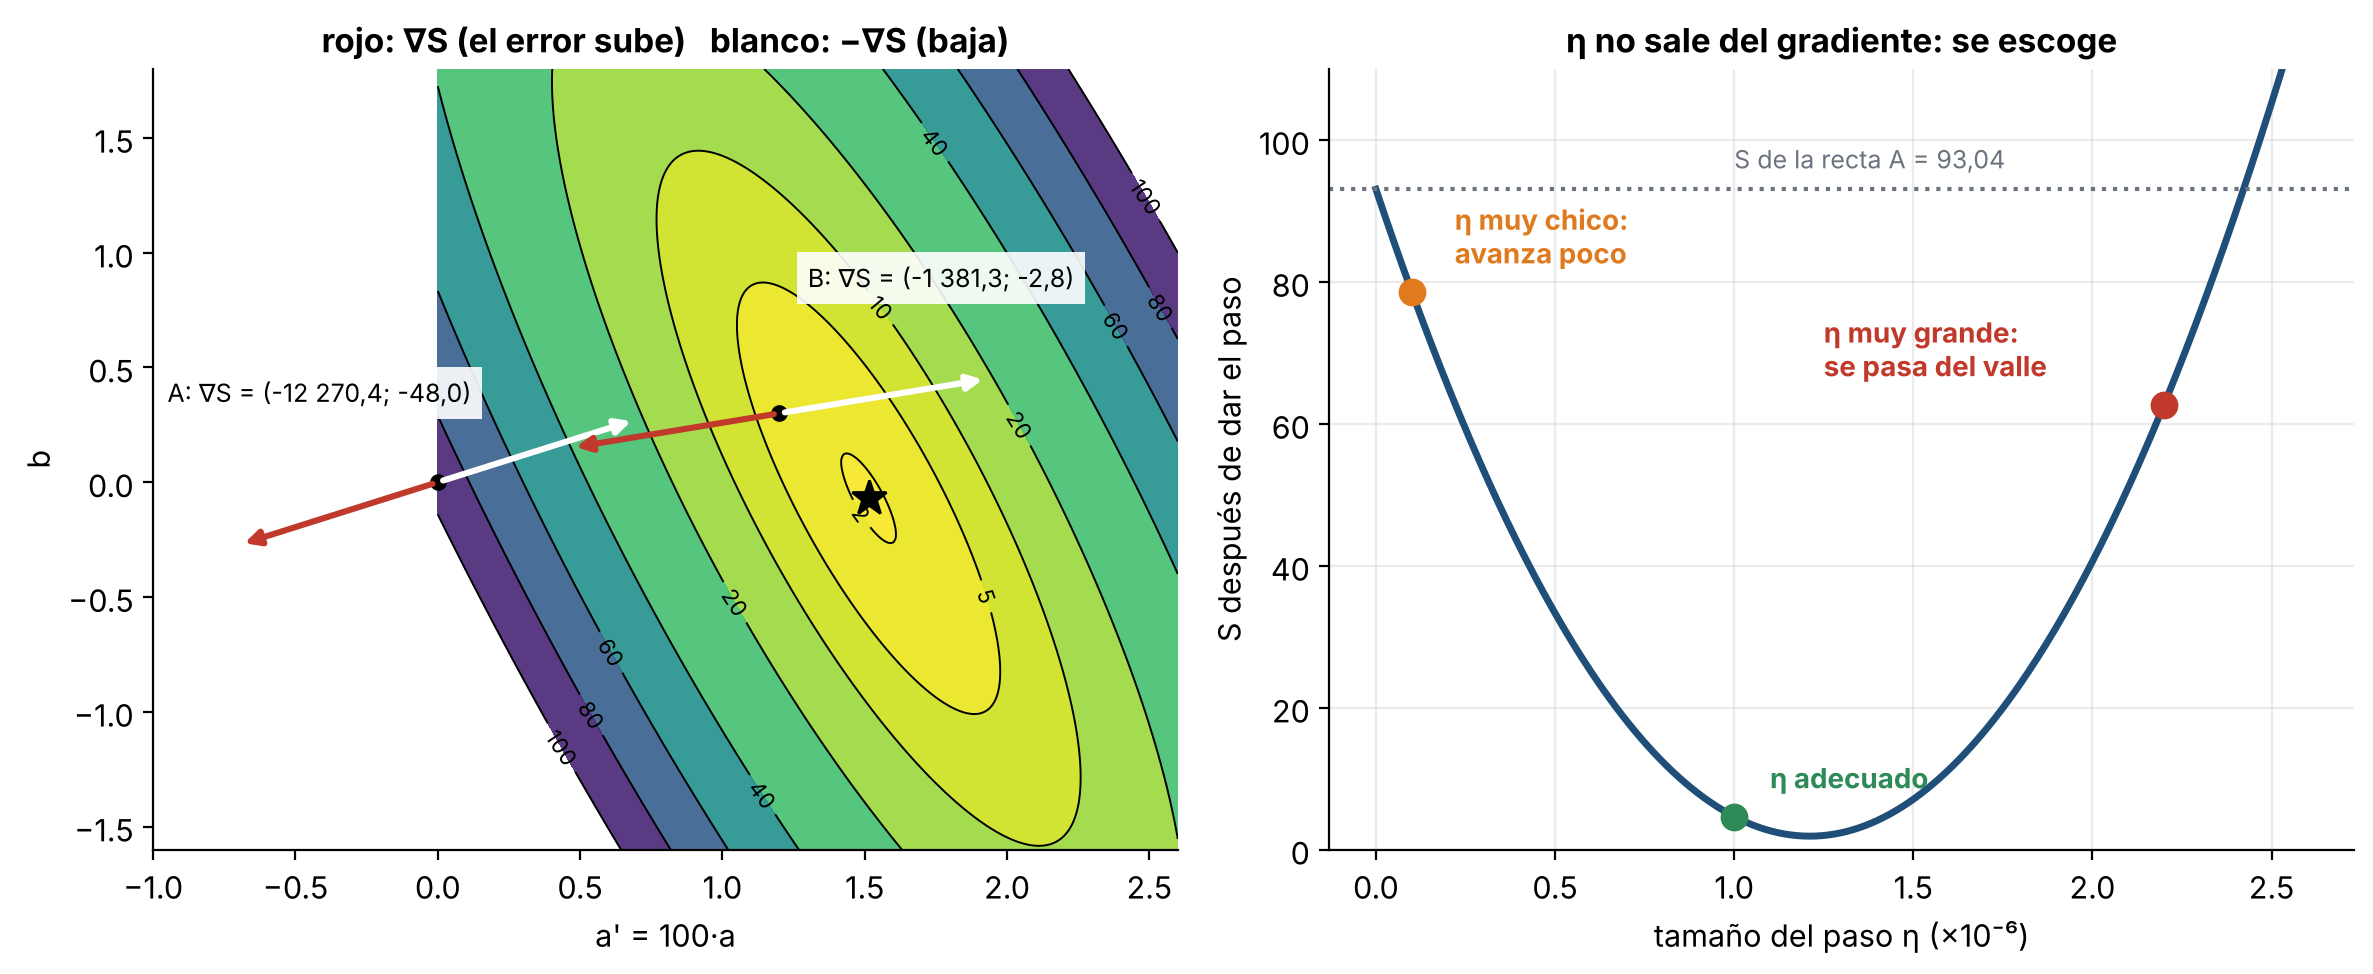
\includegraphics[width=0.9\linewidth]{11_gradiente_paso.png}\\[0.2em]
  \[ a_{\text{nuevo}}=a-\eta\,\frac{\partial S}{\partial a},\qquad b_{\text{nuevo}}=b-\eta\,\frac{\partial S}{\partial b}
     \qquad\text{(el gradiente da la dirección; $\eta$ se escoge)} \]
\end{frame}

\begin{frame}{6.4 Síntesis geométrica}
  \begin{columns}[T]
    \column{0.32\textwidth}
    \begin{block}{Superficie}
      Existe un único punto más bajo.
    \end{block}
    \column{0.32\textwidth}
    \begin{block}{Secciones}
      Desde cualquier dirección se llega a él bajando por una parábola.
    \end{block}
    \column{0.32\textwidth}
    \begin{block}{Curvas de nivel}
      Lo ubican en el plano $(a,b)$ como el centro de las elipses.
    \end{block}
  \end{columns}
  \vspace{1em}
  \begin{resultado}
    \centering Las tres representaciones señalan el mismo punto que se obtuvo con $\nabla S=0$.
  \end{resultado}
\end{frame}

% =====================================================================
\section{Verificación computacional}

\begin{frame}{7.1 Programa en Python}
  \begin{columns}[T]
    \column{0.55\textwidth}
    El programa \texttt{regresion\_hooke.py}:
    \begin{enumerate}\small
      \item carga los datos;
      \item calcula las sumas y, con las fórmulas de la sección 5, obtiene $a^*$ y $b^*$ \textbf{sin usar
            ninguna función de regresión};
      \item calcula $S(a^*,b^*)$, RMSE y $R^2$;
      \item construye todas las gráficas;
      \item calcula y verifica el Hessiano (también por diferencias finitas);
      \item solo al final compara con \texttt{numpy.polyfit}.
    \end{enumerate}
    \column{0.42\textwidth}
    \begin{block}{Nuevo en esta versión}
      \small
      \begin{itemize}
        \item intervalos de confianza de $a$, $b$, $k$;
        \item sensibilidad (quitar un dato, Monte Carlo);
        \item error de la regla y la gramera;
        \item polinomios de grado 1 a 4;
        \item RMSE en mm, g y N.
      \end{itemize}
    \end{block}
  \end{columns}
\end{frame}

\begin{frame}[fragile]{7.2 Pseudocódigo}
  \begin{columns}[T]
    \column{0.49\textwidth}
\begin{lstlisting}
ALGORITMO AjusteMinimosCuadrados
  LEER los n pares (x_i, y_i)
  // 1. Sumas (Diagrama 2)
  n <- 0; Sx <- 0; Sy <- 0
  Sxx <- 0; Sxy <- 0; Syy <- 0
  PARA CADA par (x_i, y_i) HACER
    n <- n + 1
    Sx <- Sx + x_i;      Sy <- Sy + y_i
    Sxx <- Sxx + x_i*x_i
    Sxy <- Sxy + x_i*y_i
    Syy <- Syy + y_i*y_i
  FIN PARA
  // 2. Punto critico: grad S = 0
  D <- n*Sxx - Sx*Sx
  SI D = 0 ENTONCES
    ESCRIBIR "No hay solucion unica"
    TERMINAR
  FIN SI
  a <- (n*Sxy - Sx*Sy) / D
  b <- (Sy - a*Sx) / n
\end{lstlisting}
    \column{0.49\textwidth}
\begin{lstlisting}
  // 3. Error minimo y calidad (Diagrama 3)
  S <- 0; ST <- 0; ym <- Sy / n
  PARA CADA par (x_i, y_i) HACER
    e_i <- y_i - (a*x_i + b)
    S  <- S + e_i*e_i
    ST <- ST + (y_i - ym)^2
  FIN PARA
  RMSE <- raiz(S / n);  R2 <- 1 - S/ST
  // 4. Hessiano
  H <- [[2*Sxx, 2*Sx], [2*Sx, 2*n]]
  detH <- 4*D
  SI 2*Sxx > 0 Y detH > 0 ENTONCES
    ESCRIBIR "El punto critico es un minimo"
  FIN SI
  // 5. Verificacion y salida
  (a_lib, b_lib) <- numpy.polyfit
  ESCRIBIR a, b, S, RMSE, R2, H, detH
  DIBUJAR las graficas
FIN ALGORITMO
\end{lstlisting}
  \end{columns}
\end{frame}

\begin{frame}{7.3 Diagrama de flujo general}
  \begin{columns}[c]
    \column{0.36\textwidth}
    \centering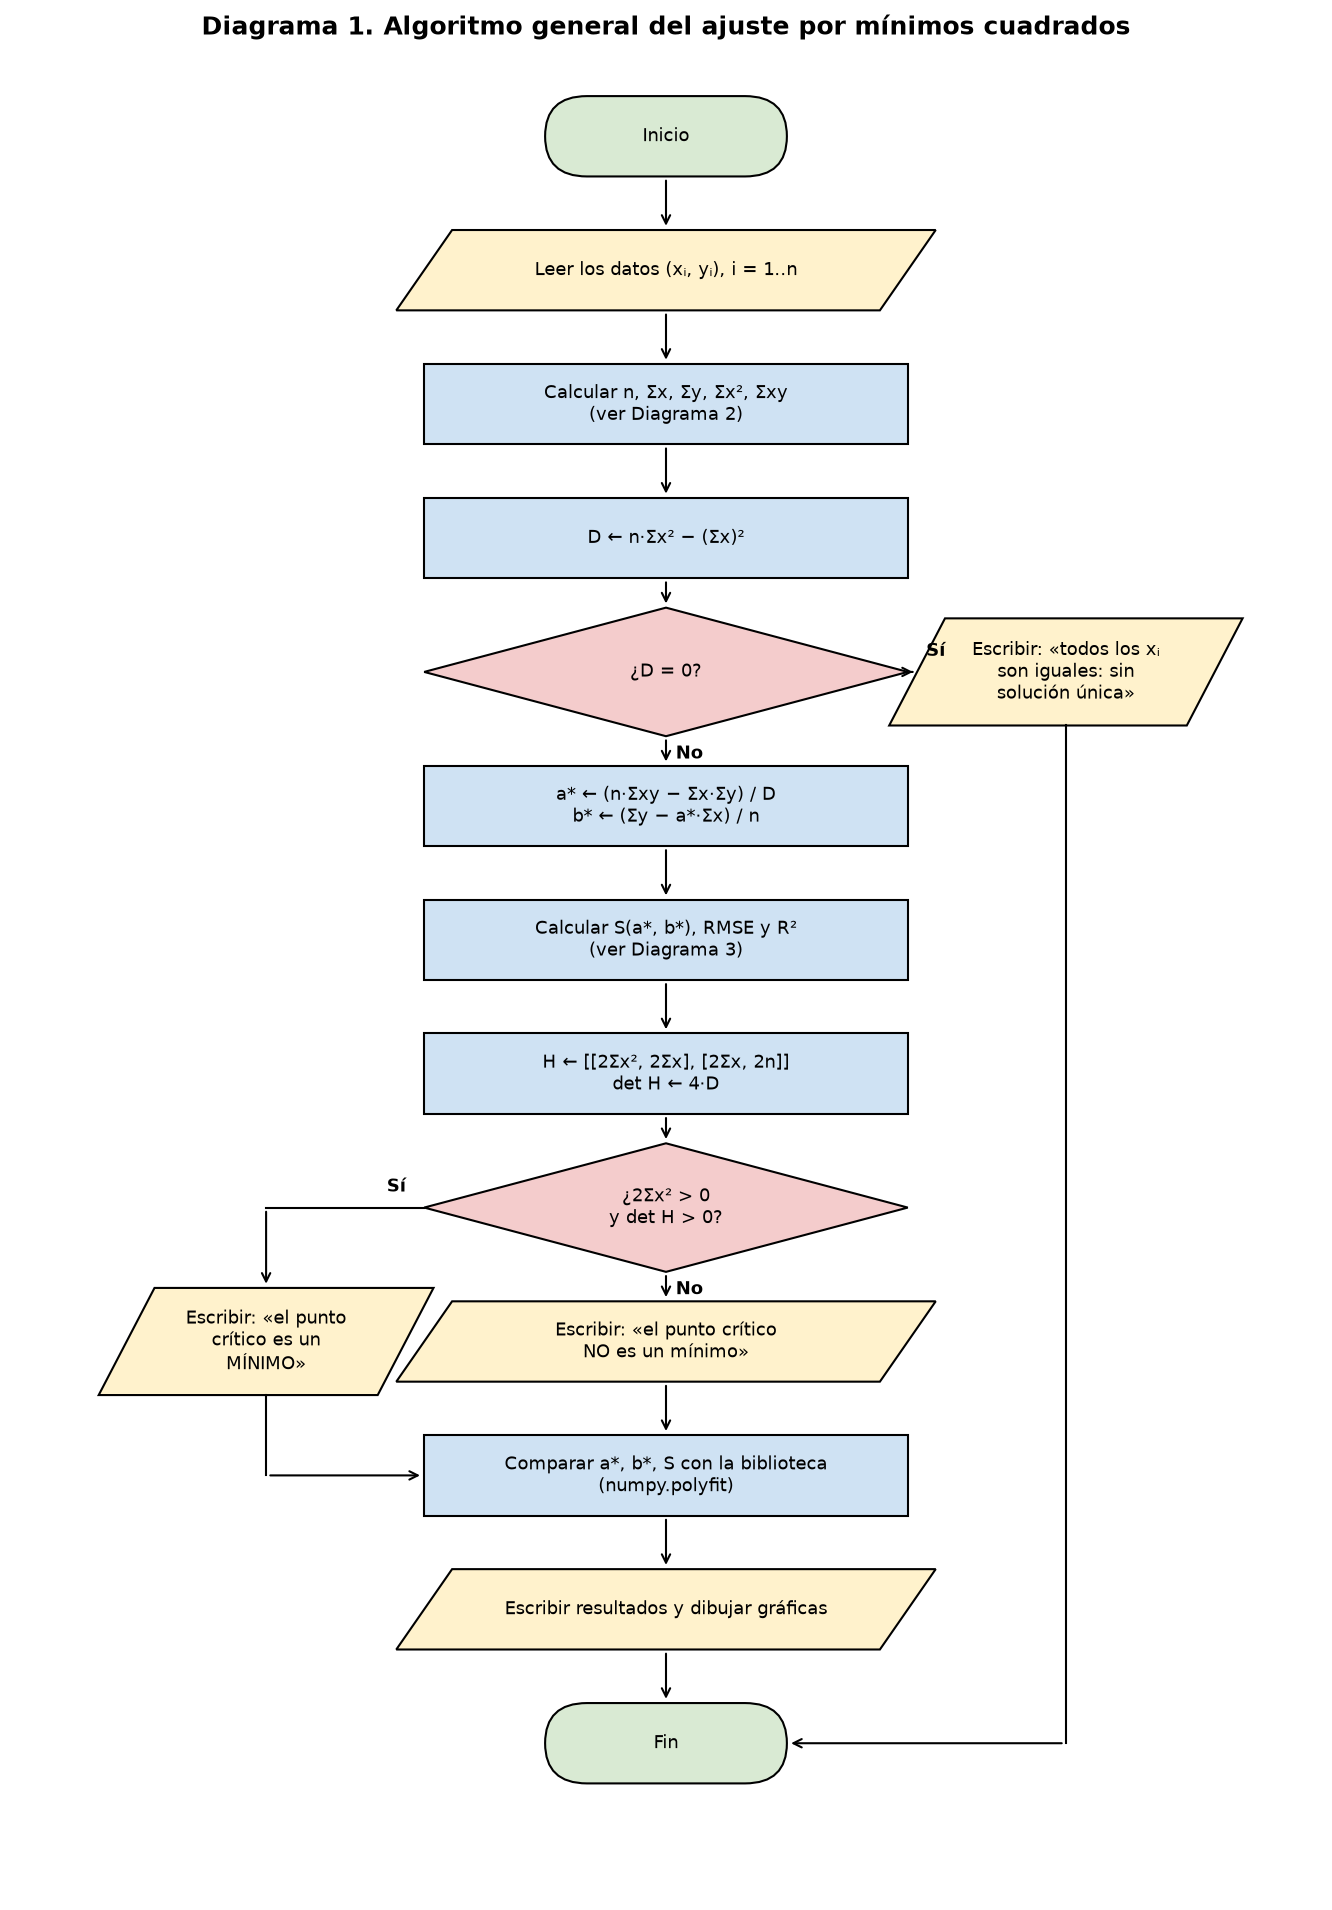
\includegraphics[height=0.8\textheight]{diagrama_1_general.png}
    \column{0.6\textwidth}
    \textbf{Lectura del diagrama}
    \begin{enumerate}\small
      \item Se leen los datos y se calculan las sumas.
      \item Se calcula $D=n\sum x^2-(\sum x)^2$. Si $D=0$ no hay solución única.
      \item Se resuelven las ecuaciones normales: $a^*$ y $b^*$.
      \item Se calculan $S$, RMSE y $R^2$.
      \item Se arma el Hessiano y se aplica el criterio de la segunda derivada.
      \item Se compara con la biblioteca y se dibujan los gráficos.
    \end{enumerate}
  \end{columns}
\end{frame}

\begin{frame}{7.4 Relación entre el código y el modelo}
  \centering\footnotesize\renewcommand{\arraystretch}{0.95}
  \begin{tabular}{ll}
    \toprule
    Modelo matemático & Código (\texttt{regresion\_hooke.py}) \\
    \midrule
    Sumas $\sum x_i,\ \sum y_i,\ \sum x_i^2,\ \sum x_iy_i$ & \texttt{sumas} \\
    Solución de $\nabla S=0$ & \texttt{ajustar} \\
    $S(a,b)=\sum(y_i-ax_i-b)^2$ & \texttt{error\_S} \\
    Hessiano $H$ & \texttt{hessiano} \\
    Residuos $e_i$ & \texttt{residuos} \\
    RMSE y $R^2$ & \texttt{calidad} \\
    \midrule
    Intervalos de confianza y bandas & \texttt{intervalos}, \texttt{banda} \\
    Sensibilidad de $k$ & \texttt{jackknife}, \texttt{montecarlo} \\
    Error de la regla y la gramera & \texttt{incertidumbre\_instrumental} \\
    Regresión polinómica & \texttt{polinomios} \\
    \bottomrule
  \end{tabular}
\end{frame}

\begin{frame}{7.5 Verificación numérica del Hessiano}
  El programa obtuvo $\det H=5\,862\,864>0$ y valores propios
  \[ \lambda_1\approx 825\,840{,}9,\qquad \lambda_2\approx 7{,}099, \]
  ambos positivos: $H$ es \textbf{definida positiva}. El Hessiano calculado por diferencias finitas coincidió
  con el analítico.
  \begin{columns}[T]
    \column{0.48\textwidth}
    \begin{block}{$\lambda_1$ grande}
      Dirección en la que el error crece muy rápido (cambiar la pendiente).
    \end{block}
    \column{0.48\textwidth}
    \begin{block}{$\lambda_2$ pequeño}
      Dirección en la que crece despacio: el eje largo de las elipses.
    \end{block}
  \end{columns}
\end{frame}

\begin{frame}{7.6 Recta ajustada y otras rectas}
  \begin{columns}[c]
    \column{0.6\textwidth}
    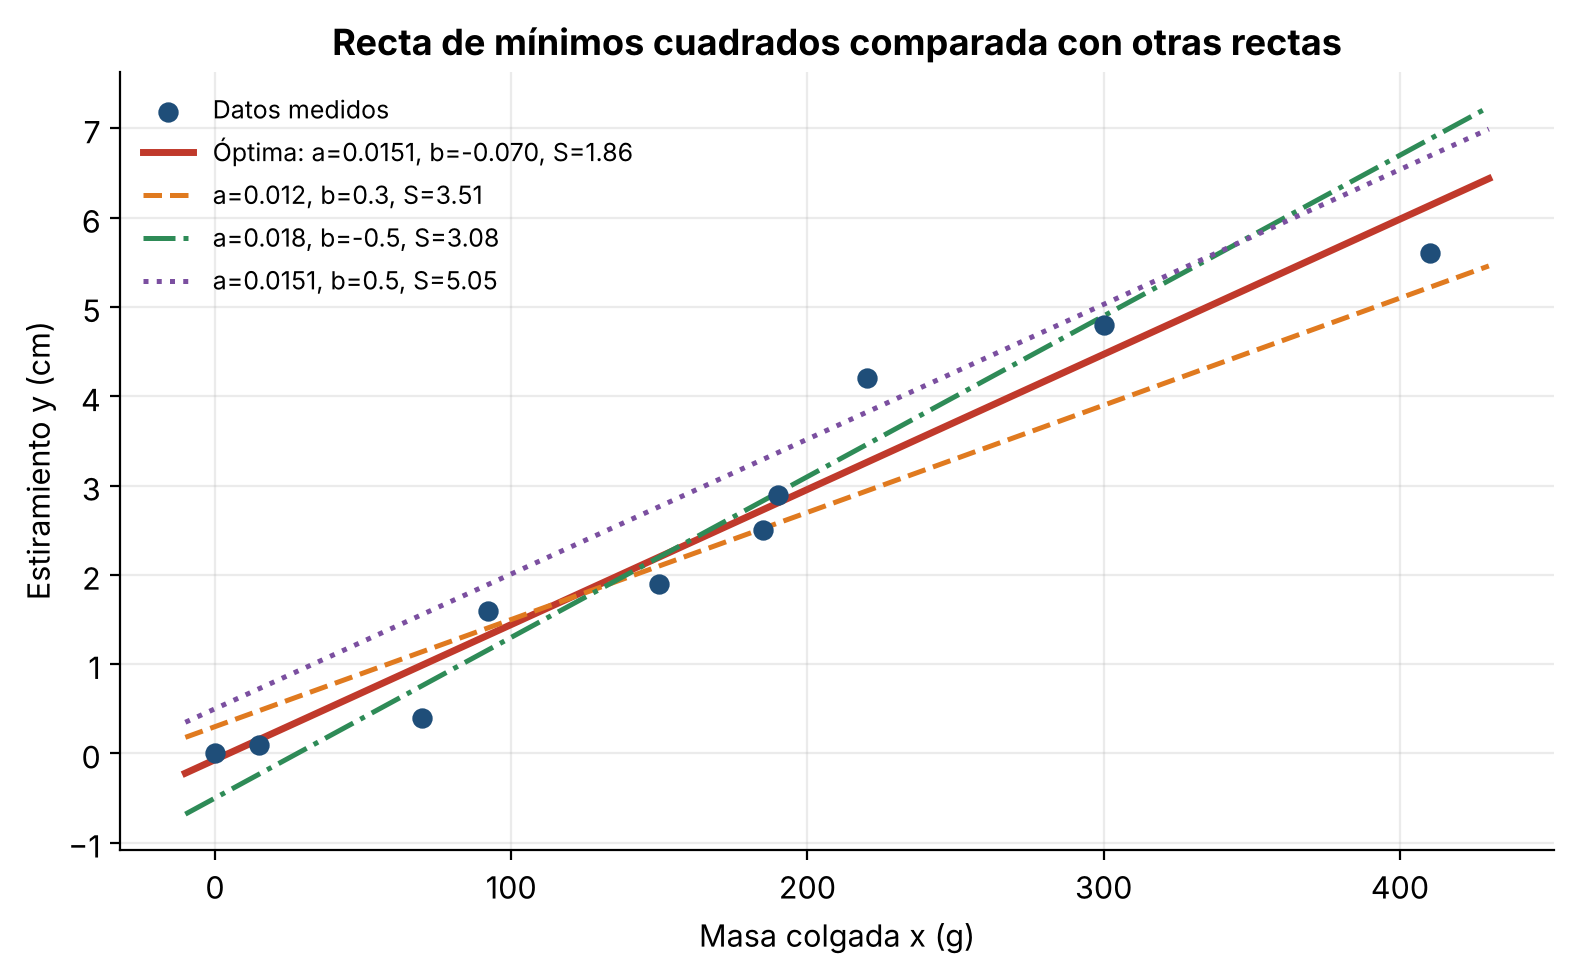
\includegraphics[width=\linewidth]{02_recta_ajuste.png}
    \column{0.38\textwidth}
    \centering\small
    \begin{tabular}{lrrr}
      \toprule
      Recta & $a$ & $b$ & $S$ \\
      \midrule
      \textbf{Óptima} & \textbf{0,0151} & $\mathbf{-0{,}070}$ & \textbf{1,86} \\
      Prueba 1 & 0,012 & 0,3 & 3,51 \\
      Prueba 2 & 0,018 & $-0{,}5$ & 3,08 \\
      Prueba 3 & 0,0151 & 0,5 & 5,05 \\
      \bottomrule
    \end{tabular}
    \begin{resultado}[fontupper=\small]
      Ninguna pareja $(a,b)$ da menos de 1,86 cm$^2$: es el mínimo global de $S$.
    \end{resultado}
  \end{columns}
\end{frame}

% =====================================================================
\section{Comparación analítico--computacional}

\begin{frame}{8. Comparación entre el procedimiento analítico y el computacional}
  \centering
  \begin{tabular}{lrrrr}
    \toprule
    Parámetro & Analítico (a mano) & Código propio & Biblioteca (\texttt{polyfit}) & Dif. máx. \\
    \midrule
    $a$ (cm/g) & 0,0151353 & 0,0151353 & 0,0151353 & $3{,}5\times10^{-8}$ \\
    $b$ (cm) & $-0{,}0700810$ & $-0{,}0700752$ & $-0{,}0700752$ & $5{,}8\times10^{-6}$ \\
    $S_{\min}$ (cm$^2$) & 1,8639000 & 1,8639282 & 1,8639282 & $2{,}8\times10^{-5}$ \\
    \bottomrule
  \end{tabular}
  \vspace{0.8em}
  \begin{resultado}[fontupper=\small]
    Los tres métodos coinciden. La pequeña diferencia de la columna manual se debe al redondeo (7 decimales en
    $a^*$, 4 en los residuos); es miles de veces menor que la resolución de la regla (0,1 cm).
  \end{resultado}
\end{frame}

% =====================================================================
\section{Análisis de la recta y de los residuos}

\begin{frame}{9. Análisis de la recta de ajuste}
  La recta $y=0{,}0151x-0{,}070$ representa bien la tendencia general: sube con los datos y deja puntos a ambos
  lados.
  \begin{itemize}\small
    \item \textbf{Mayor desviación:} parlante (220 g), residuo $+0{,}94$ cm; tornillo (70 g), $-0{,}59$ cm;
          alicate (410 g), $-0{,}54$ cm.
    \item \textbf{Punto alejado:} el parlante se estiró más de lo que predice la recta; es el candidato a dato
          atípico (sección 12).
    \item \textbf{Punto con más palanca:} el alicate (410 g) es la masa más alejada y controla más la pendiente
          (al quitarlo, $k$ cambia más que con cualquier otro dato: sección 11).
    \item \textbf{Intercepto:} $b^*=-0{,}070$ cm es menor que la resolución de la regla y su intervalo de
          confianza contiene el 0: prácticamente cero, como predice Hooke.
  \end{itemize}
\end{frame}

\begin{frame}{10. Análisis de los residuos}
  \centering
  \begin{columns}[c]
    \column{0.56\textwidth}
    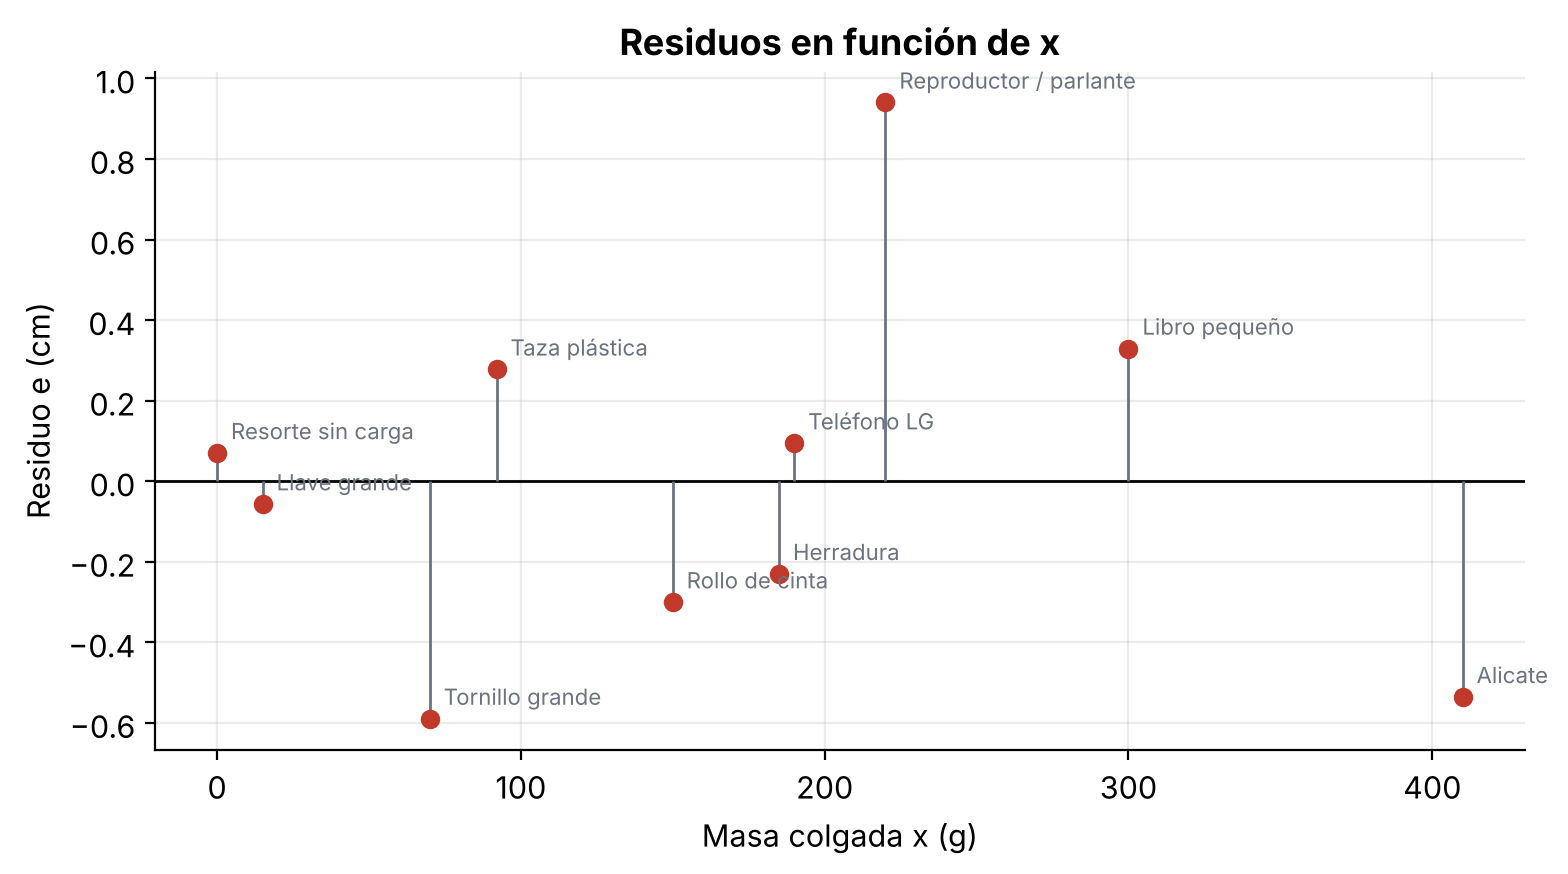
\includegraphics[width=\linewidth]{06_residuos.png}
    \column{0.42\textwidth}
    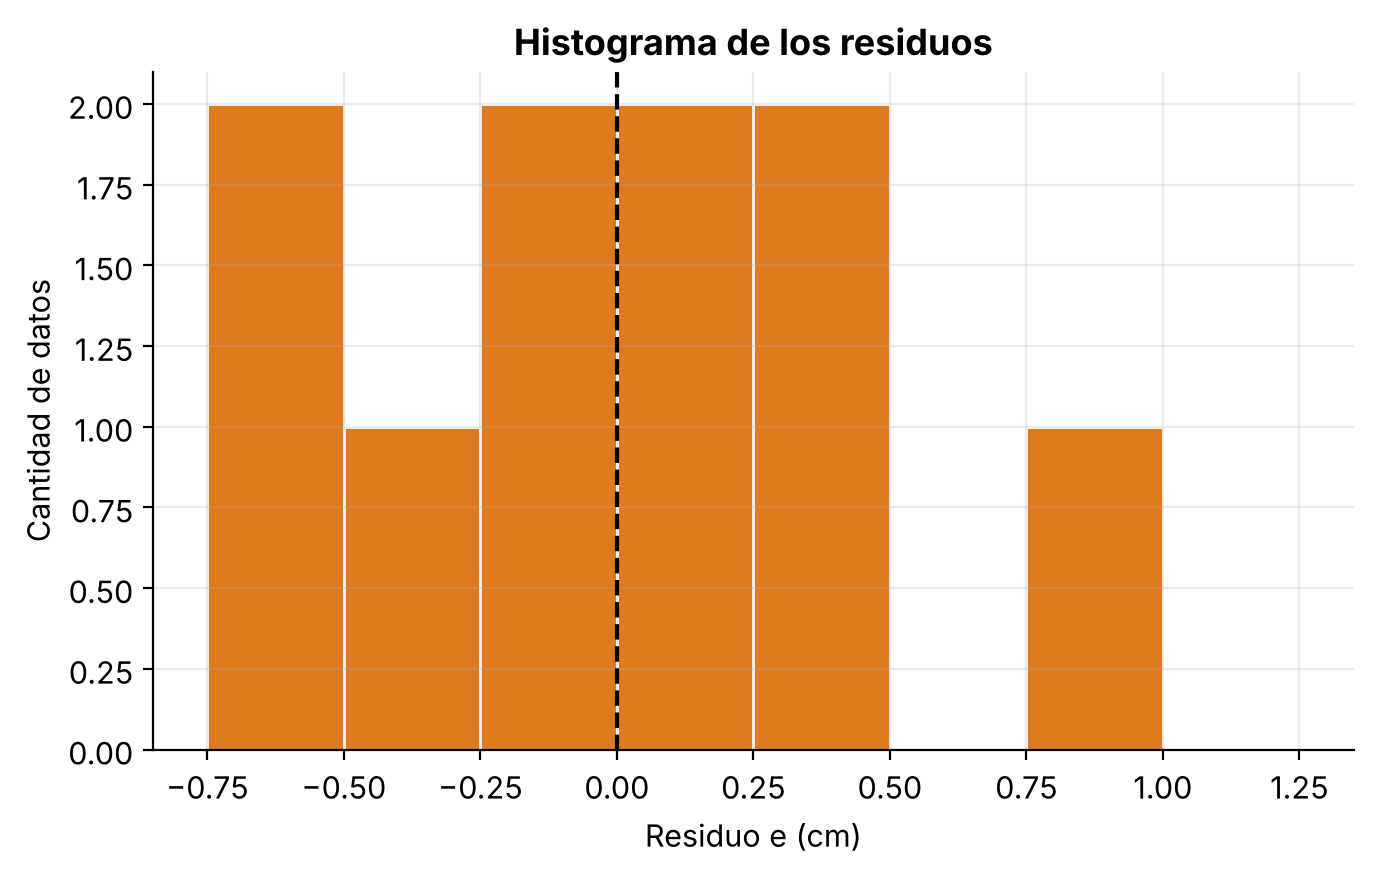
\includegraphics[width=\linewidth]{07_histograma.png}
  \end{columns}
  \vspace{0.3em}
  {\small 5 residuos positivos y 5 negativos que suman cero (consecuencia de $\partial S/\partial b=0$). El parlante
  es el único que se separa del grupo.}
\end{frame}

\begin{frame}{10. Análisis de los residuos (cont.)}
  \small
  \begin{itemize}
    \item \textbf{Centrados en cero:} sí. La suma es cero salvo redondeo.
    \item \textbf{Tendencia:} los signos se alternan sin orden claro; indicio leve: negativos en 70 g y 410 g,
          positivos entre 190 g y 300 g. Con 10 datos no se puede afirmar una desviación sistemática
          (la prueba con polinomios de la sección 11 lo confirma).
    \item \textbf{Dispersión:} no aumenta ni disminuye de forma ordenada con $x$.
    \item \textbf{Atípicos:} el parlante (0,94 cm). Los otros nueve están entre $-0{,}6$ y $+0{,}4$ cm.
    \item \textbf{Cargas livianas:} el resorte se estira menos de lo que indica la pendiente; posible tensión
          inicial de las espiras.
  \end{itemize}
  \begin{resultado}[fontupper=\small]
    El comportamiento es compatible con un modelo lineal: las desviaciones se explican mejor por la forma de medir
    que por una falla del modelo.
  \end{resultado}
\end{frame}

% =====================================================================
\section{Calidad del modelo}

\begin{frame}{10.1 Evaluación de la calidad del modelo}
  \begin{columns}[T]
    \column{0.49\textwidth}
    \[ \text{RMSE}=\sqrt{\frac{1}{n}\sum e_i^2}=\sqrt{\frac{1{,}8639}{10}}=0{,}43\ \text{cm} \]
    Error típico de la recta: el estiramiento medido se aparta unos 0,43 cm del predicho.
    \column{0.49\textwidth}
    \[ R^2=1-\frac{\sum (y_i-\hat y_i)^2}{\sum (y_i-\bar y)^2}=1-\frac{1{,}8639}{35{,}44}=0{,}9474 \]
    Usar la masa elimina el 94,7\,\% del error de la mejor recta horizontal $y=\bar y$.
  \end{columns}
  \vspace{0.6em}
  \begin{resultado}[fontupper=\small]
    \textbf{Relación con el propósito:} el ajuste es adecuado para describir la tendencia y estimar $k$; para
    predecir el estiramiento de un objeto concreto es limitado, porque 0,43 cm es grande cuando el estiramiento es
    de 1 o 2 cm.
  \end{resultado}
\end{frame}

\begin{frame}{10.2 El RMSE en las unidades del fenómeno \hfill\recom}
  \centering
  \begin{tabular}{ccccc}
    \dato{\vrmseMm\ mm}{de estiramiento} &
    \dato{$\approx$ \vrmseG\ g}{de masa equivalente} &
    \dato{$\approx$ \vrmseN\ N}{de fuerza equivalente} &
    \dato{\vrmseRango\,\%}{del rango de $y$} &
    \dato{\vrmseRes\,$\times$}{la resolución de la regla}
  \end{tabular}
  \vspace{0.8em}
  \begin{columns}[T]
    \column{0.5\textwidth}\small
    \begin{itemize}
      \item \textbf{En longitud:} la recta se equivoca en promedio \vrmseMm\ mm por medición.
      \item \textbf{En masa:} como $a=0{,}0151$ cm/g, ese error equivale a no saber la masa con una
            precisión mejor que unos \vrmseG\ g (el peso de una llave grande y media).
      \item \textbf{En fuerza:} $\vrmseG\ \text{g}\times 9{,}8\ \text{m/s}^2\approx\vrmseN$ N.
    \end{itemize}
    \column{0.46\textwidth}\small
    \begin{itemize}
      \item Frente al estiramiento promedio (2,4 cm) es un \vrmseMedia\,\%.
      \item El error estándar con $n-2$ grados de libertad es $s=\vsReg$ cm (se usa en los intervalos de
            confianza).
    \end{itemize}
    \begin{nota}
      Un error de \vrmseMm\ mm es pequeño para 5,6 cm (alicate), pero grande para 0,4 cm (tornillo).
    \end{nota}
  \end{columns}
\end{frame}

% =====================================================================
\section{Incertidumbre, sensibilidad y otros modelos}

\begin{frame}{11.1 Errores de los instrumentos: regla y gramera \hfill\recom}
  \footnotesize
  \begin{columns}[T]
    \column{0.5\textwidth}
    \begin{block}{Regla de madera (resolución 0,1 cm)}
      Error de hasta $\pm 0{,}05$ cm por lectura. Incertidumbre estándar (distribución uniforme):
      \[ u_{\text{lect}}=\frac{0{,}1}{2\sqrt3}=\vuLect\ \text{cm} \]
      $y=\text{lectura total}-\text{largo}-L_0$ usa \textbf{tres lecturas}:
      \[ u_y=\sqrt3\;u_{\text{lect}}=\vuY\ \text{cm} \]
      Peor caso (los tres errores se suman): $|\Delta y|_{\max}=3(0{,}05)=\veMaxY$ cm.
    \end{block}
    \column{0.46\textwidth}
    \begin{block}{Gramera (resolución 1 g)}
      \[ u_x=\frac{1}{2\sqrt3}=\vuX\ \text{g},\qquad |\Delta x|_{\max}=\veMaxX\ \text{g} \]
      Efecto sobre $y$: $a\,u_x=\vuXy$ cm, \textbf{despreciable}.
    \end{block}
    \begin{block}{Propagación a $k=g/a$}
      \[ \frac{u_k}{k}=\frac{u_a}{a}\quad\Rightarrow\quad u_k=\vuK\ \text{N/m} \]
    \end{block}
  \end{columns}
\end{frame}

\begin{frame}{11.2 ¿El error viene de los instrumentos?}
  \begin{columns}[c]
    \column{0.52\textwidth}
    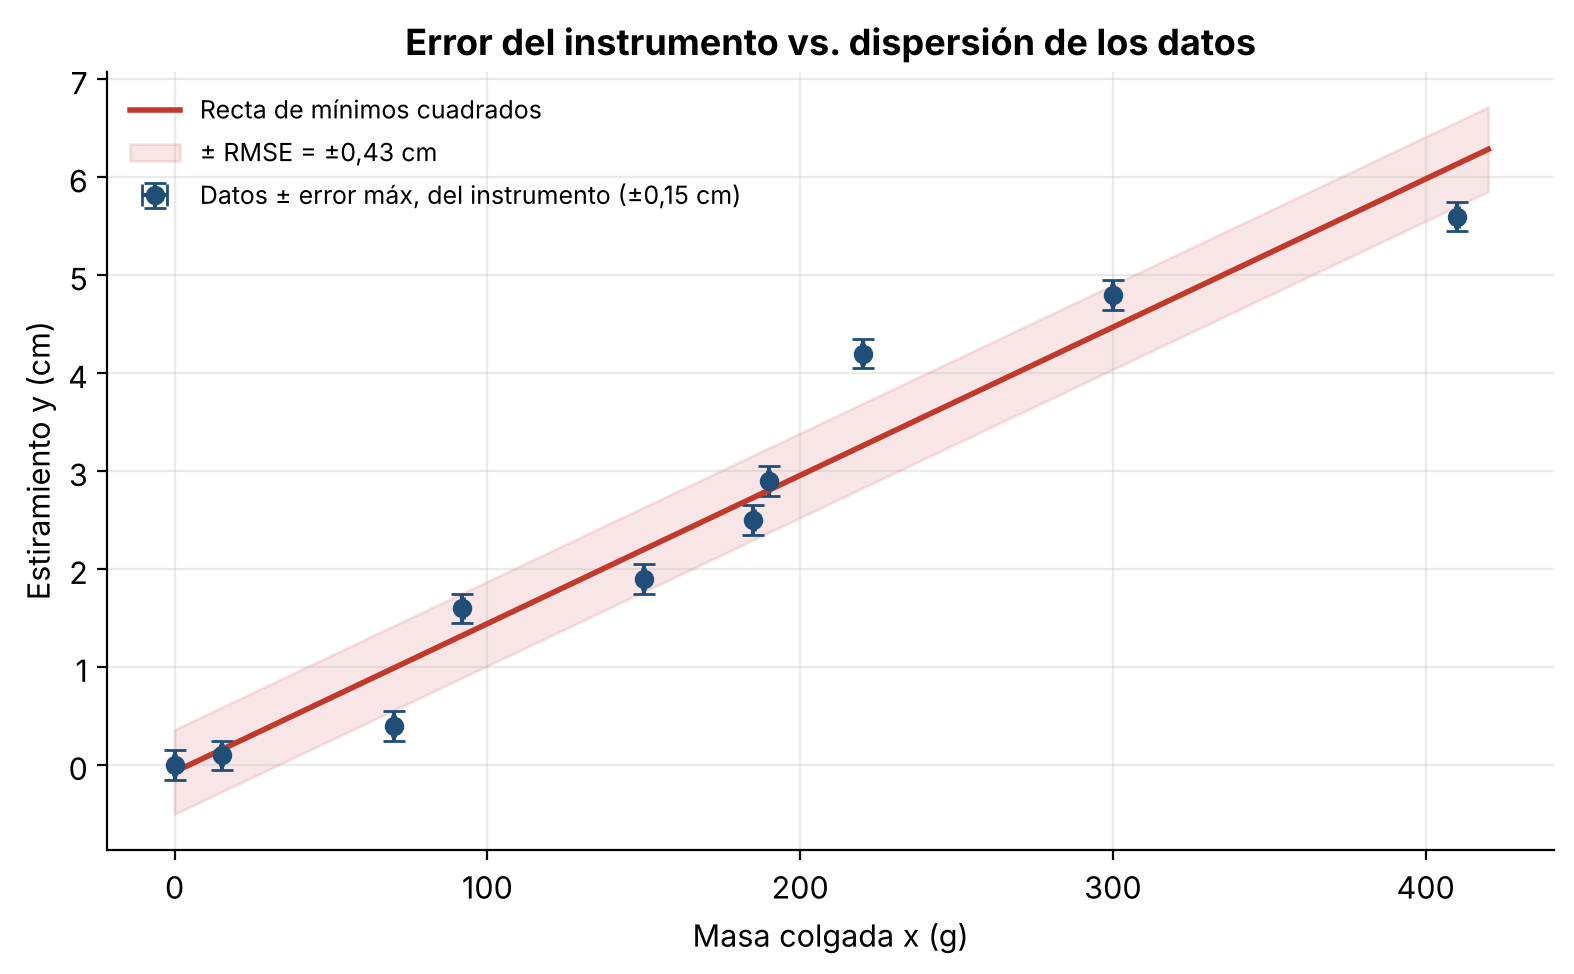
\includegraphics[width=\linewidth]{12_incertidumbre.png}
    \column{0.46\textwidth}
    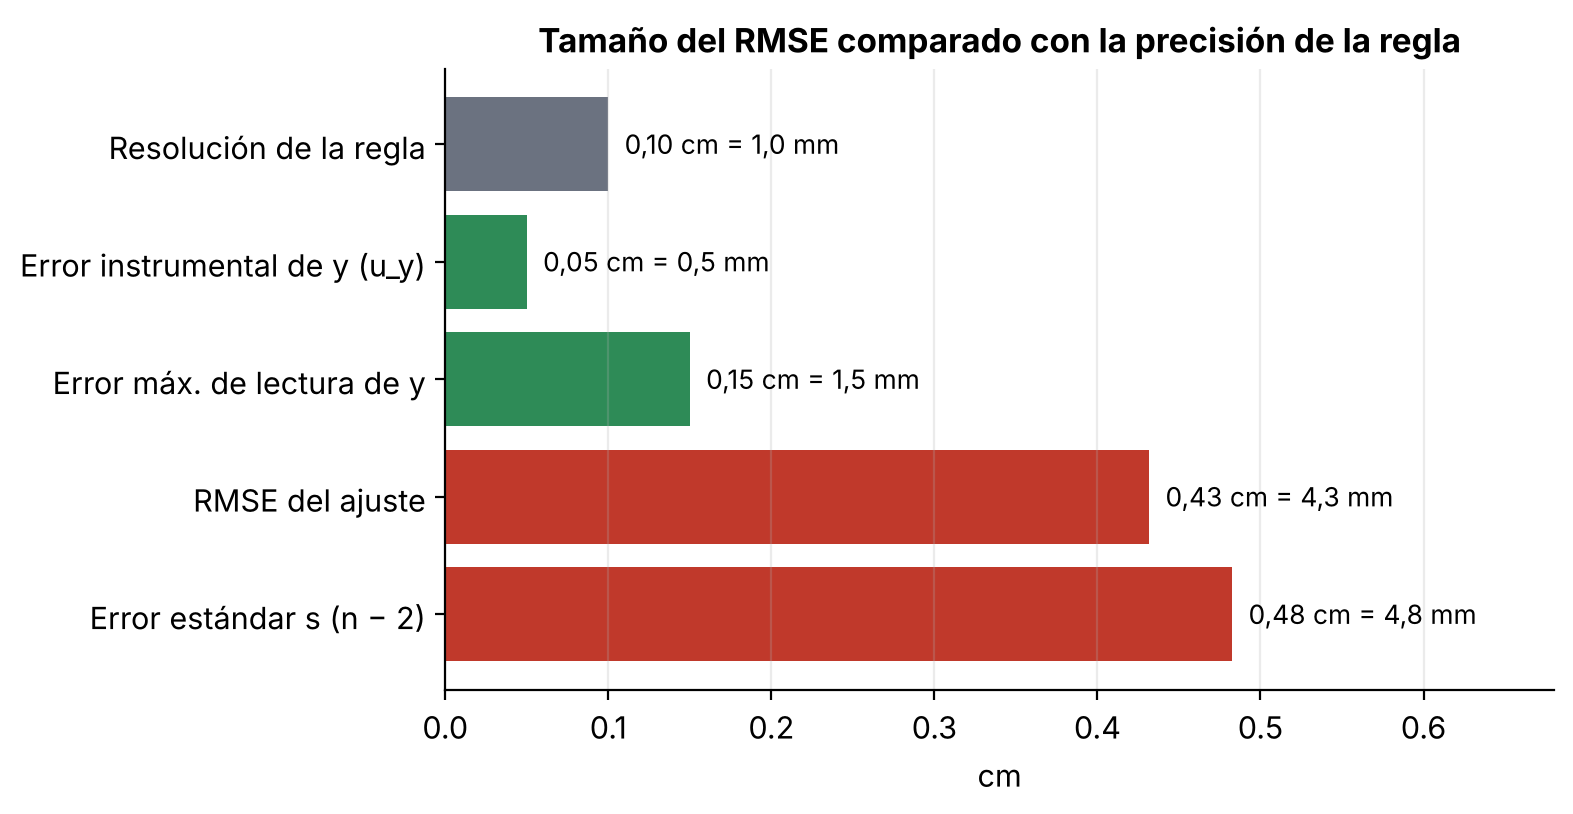
\includegraphics[width=0.9\linewidth]{16_rmse_escala.png}
    \begin{resultado}[fontupper=\footnotesize]
      $\text{RMSE}/u_y\approx\vrazon$: la dispersión es unas \textbf{\vrazon\ veces} mayor que el error de los
      instrumentos. Las barras de error ($\pm\veMaxY$ cm) no alcanzan la recta en varios puntos.
    \end{resultado}
  \end{columns}
  {\footnotesize La causa principal es el \textbf{método}: objetos de formas distintas, punto de enganche y
  restas de longitudes.}
\end{frame}

\begin{frame}{11.3 Intervalos de confianza de los parámetros \hfill\recom}
  \small
  Con $s=\sqrt{S/(n-2)}=\vsReg$ cm y $t_{0{,}975;\,8}=\vtCrit$:
  \[ SE(a)=\frac{s}{\sqrt{\sum (x_i-\bar x)^2}},\qquad SE(b)=s\sqrt{\frac1n+\frac{\bar x^2}{\sum (x_i-\bar x)^2}},
     \qquad \text{IC}_{95\,\text{\%}}=\text{valor}\pm t\cdot SE \]
  \centering
  \begin{tabular}{lcccc}
    \toprule
    Parámetro & Estimado & Error estándar & \textbf{Mínimo} (95\,\%) & \textbf{Máximo} (95\,\%) \\
    \midrule
    $a$ (cm/g) & \vaCI & \vseA & \vaLo & \vaHi \\
    $b$ (cm)   & $\vbCI$ & \vseB & $\vbLo$ & \vbHi \\
    \rowcolor{azulclaro}
    $k$ (N/m)  & \vkVal & \vuK & \vkLo & \vkHi \\
    \bottomrule
  \end{tabular}
  \vspace{0.5em}
  \begin{columns}[T]
    \column{0.49\textwidth}
    \begin{resultado}[fontupper=\small]
      El intervalo de $b$ \textbf{contiene el 0}: los datos son compatibles con $y=ax$, como dice Hooke.
    \end{resultado}
    \column{0.49\textwidth}
    \begin{nota}
      $k$ está entre \vkLo\ y \vkHi\ N/m (amplitud \vkRango\ N/m). Como $k=g/a$, el intervalo de $k$ no es
      simétrico.
    \end{nota}
  \end{columns}
\end{frame}

\begin{frame}{11.4 Bandas de confianza y de predicción}
  \begin{columns}[c]
    \column{0.58\textwidth}
    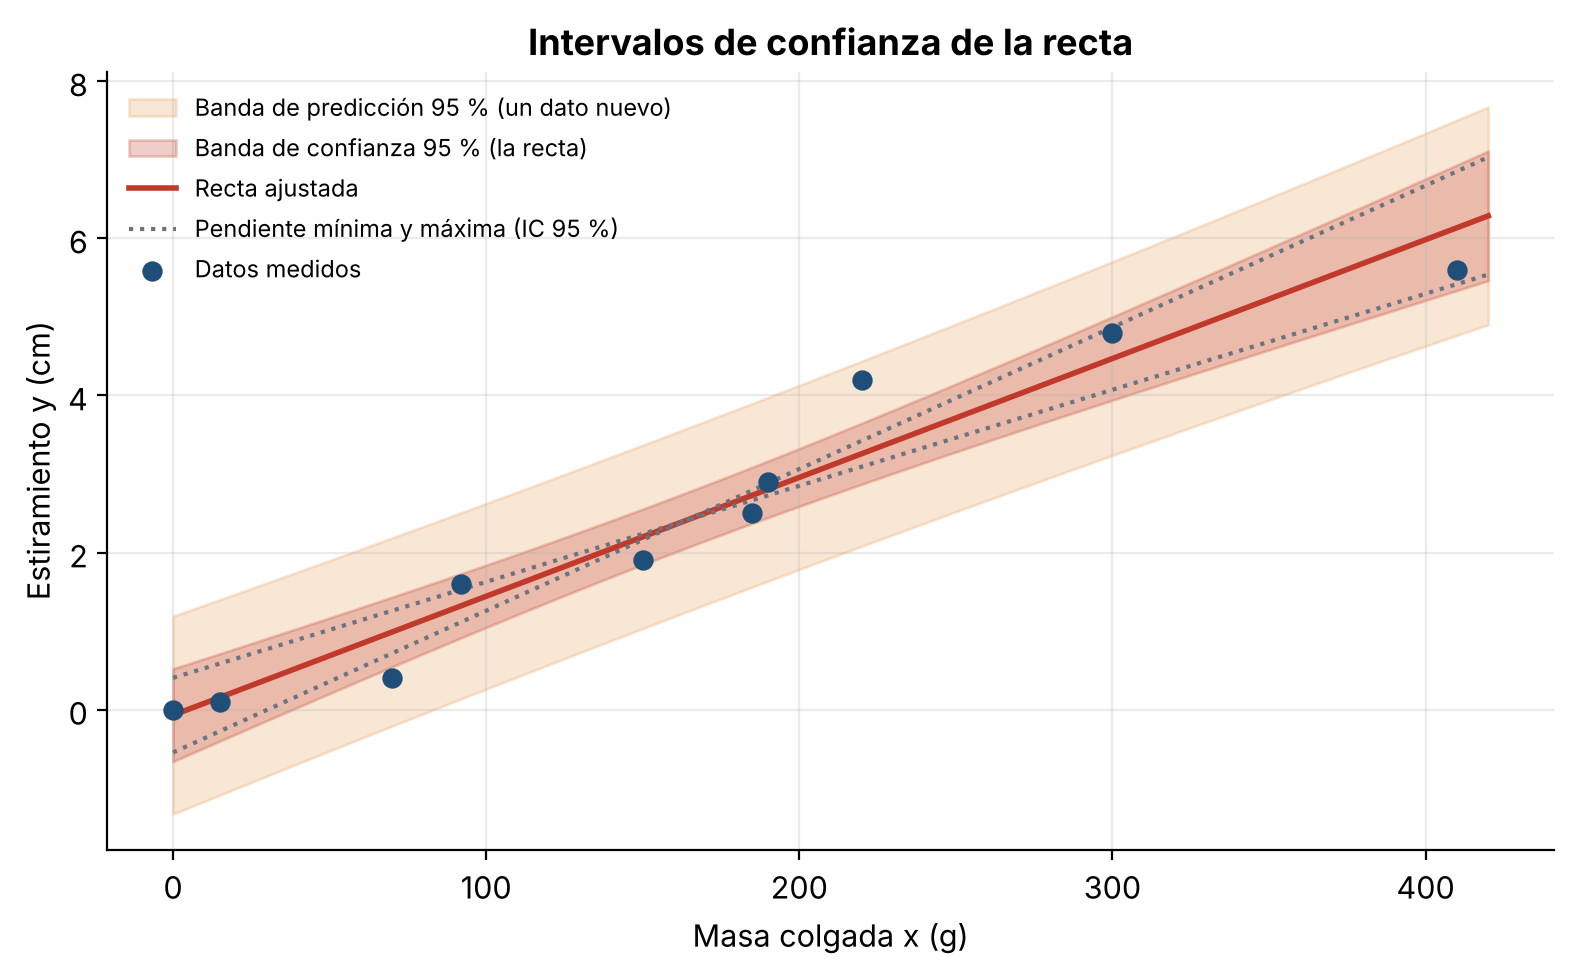
\includegraphics[width=\linewidth]{13_bandas_confianza.png}
    \column{0.4\textwidth}\small
    \begin{block}{Banda de confianza (roja)}
      Dónde está la \emph{recta verdadera}. En $x=200$ g: $\pm\vbandaC$ cm.
    \end{block}
    \begin{block}{Banda de predicción (naranja)}
      Dónde caería \emph{una medición nueva}. En $x=200$ g: $\pm\vbandaP$ cm.
    \end{block}
    Las bandas se abren en los extremos: la recta es más segura cerca de $\bar x=163$ g.
  \end{columns}
\end{frame}

\begin{frame}{11.5 Sensibilidad: valor mínimo y máximo de $k$ \hfill\recom}
  \centering
  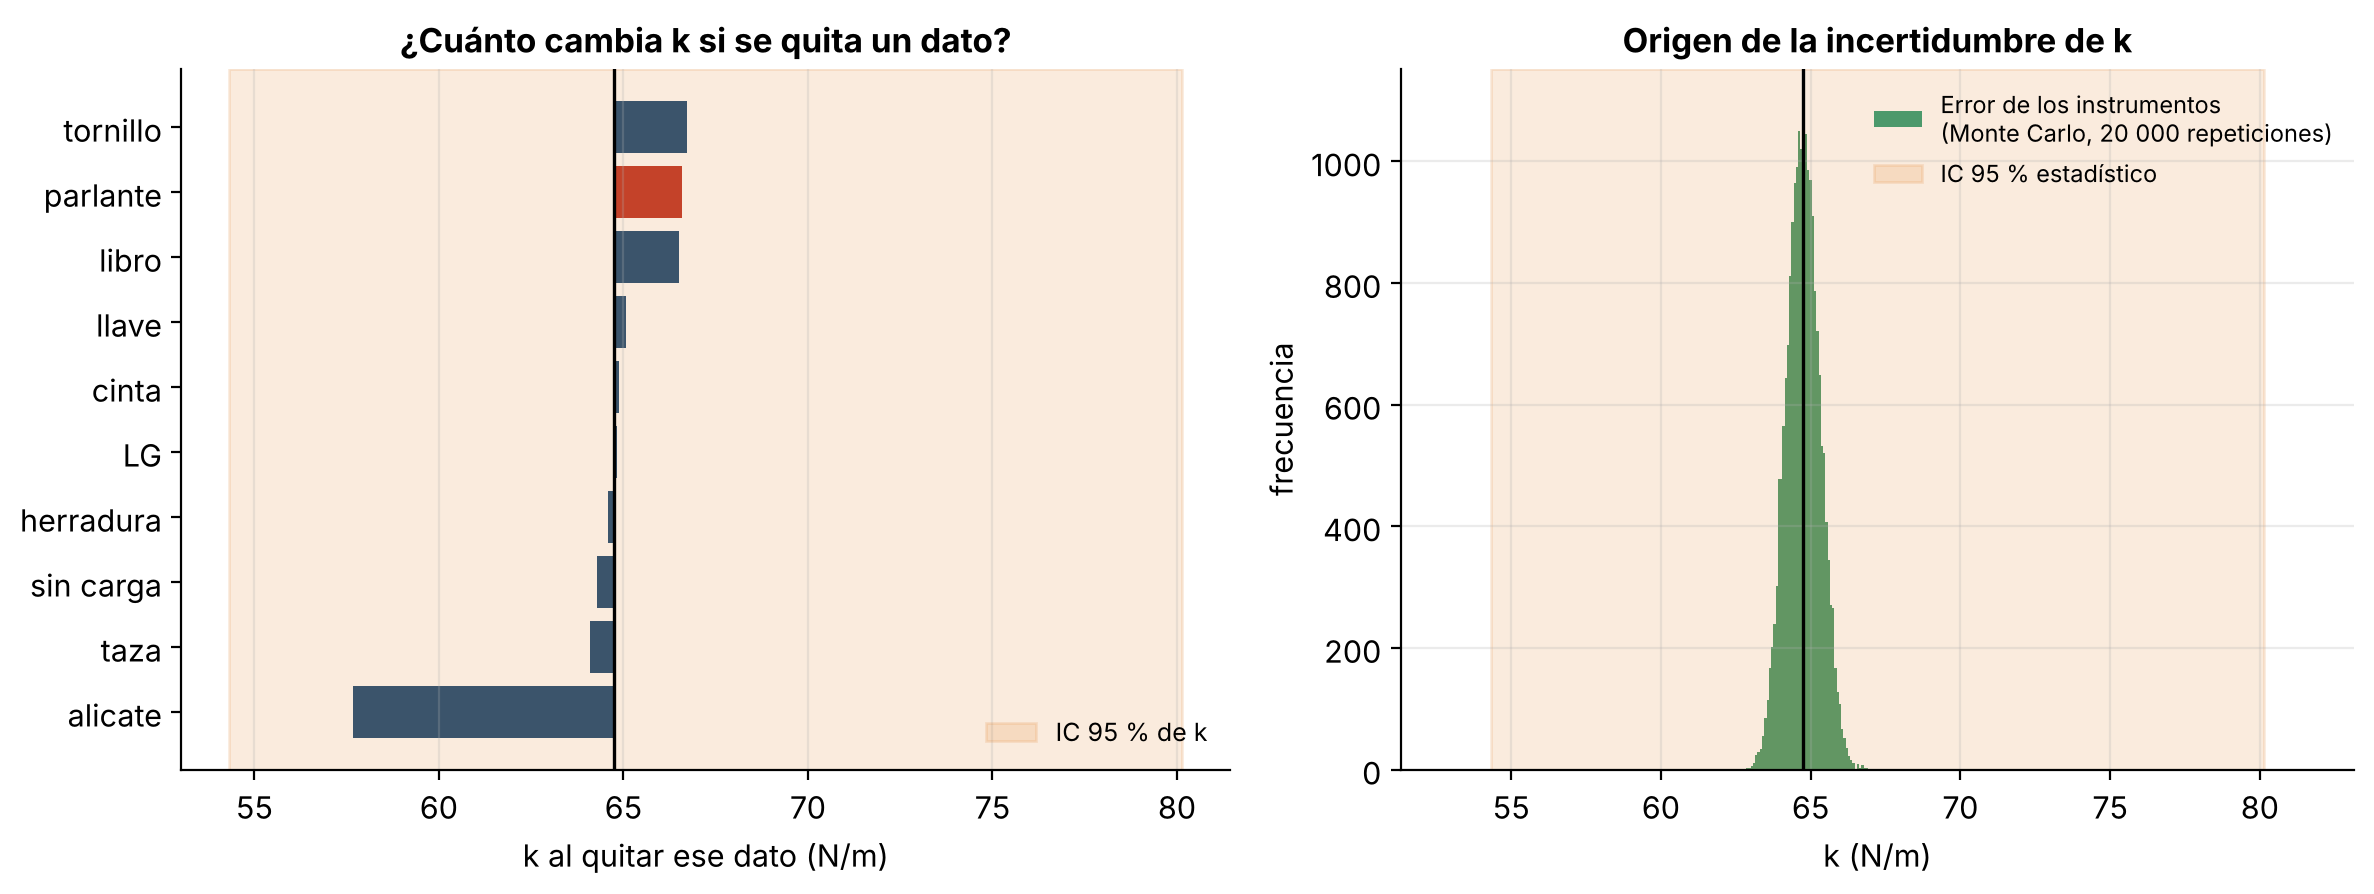
\includegraphics[width=0.9\linewidth]{14_sensibilidad_k.png}
  \vspace{0.1em}
  \begin{columns}[T]
    \column{0.49\textwidth}\footnotesize
    \textbf{Quitando un dato a la vez}, $k$ varía entre \textbf{\vjkMin} (sin el \vjkMinObj) y \textbf{\vjkMax} N/m
    (sin el \vjkMaxObj). El alicate es el dato con más palanca.
    \column{0.49\textwidth}\footnotesize
    \textbf{Error de los instrumentos} (Monte Carlo): $k$ solo varía entre \vmcLo\ y \vmcHi\ N/m. La
    incertidumbre de $k$ viene de la dispersión de los datos, no de la regla ni de la gramera.
  \end{columns}
\end{frame}

\begin{frame}{11.6 ¿Se ajusta mejor otra función? Regresión polinómica \hfill\recom}
  \centering
  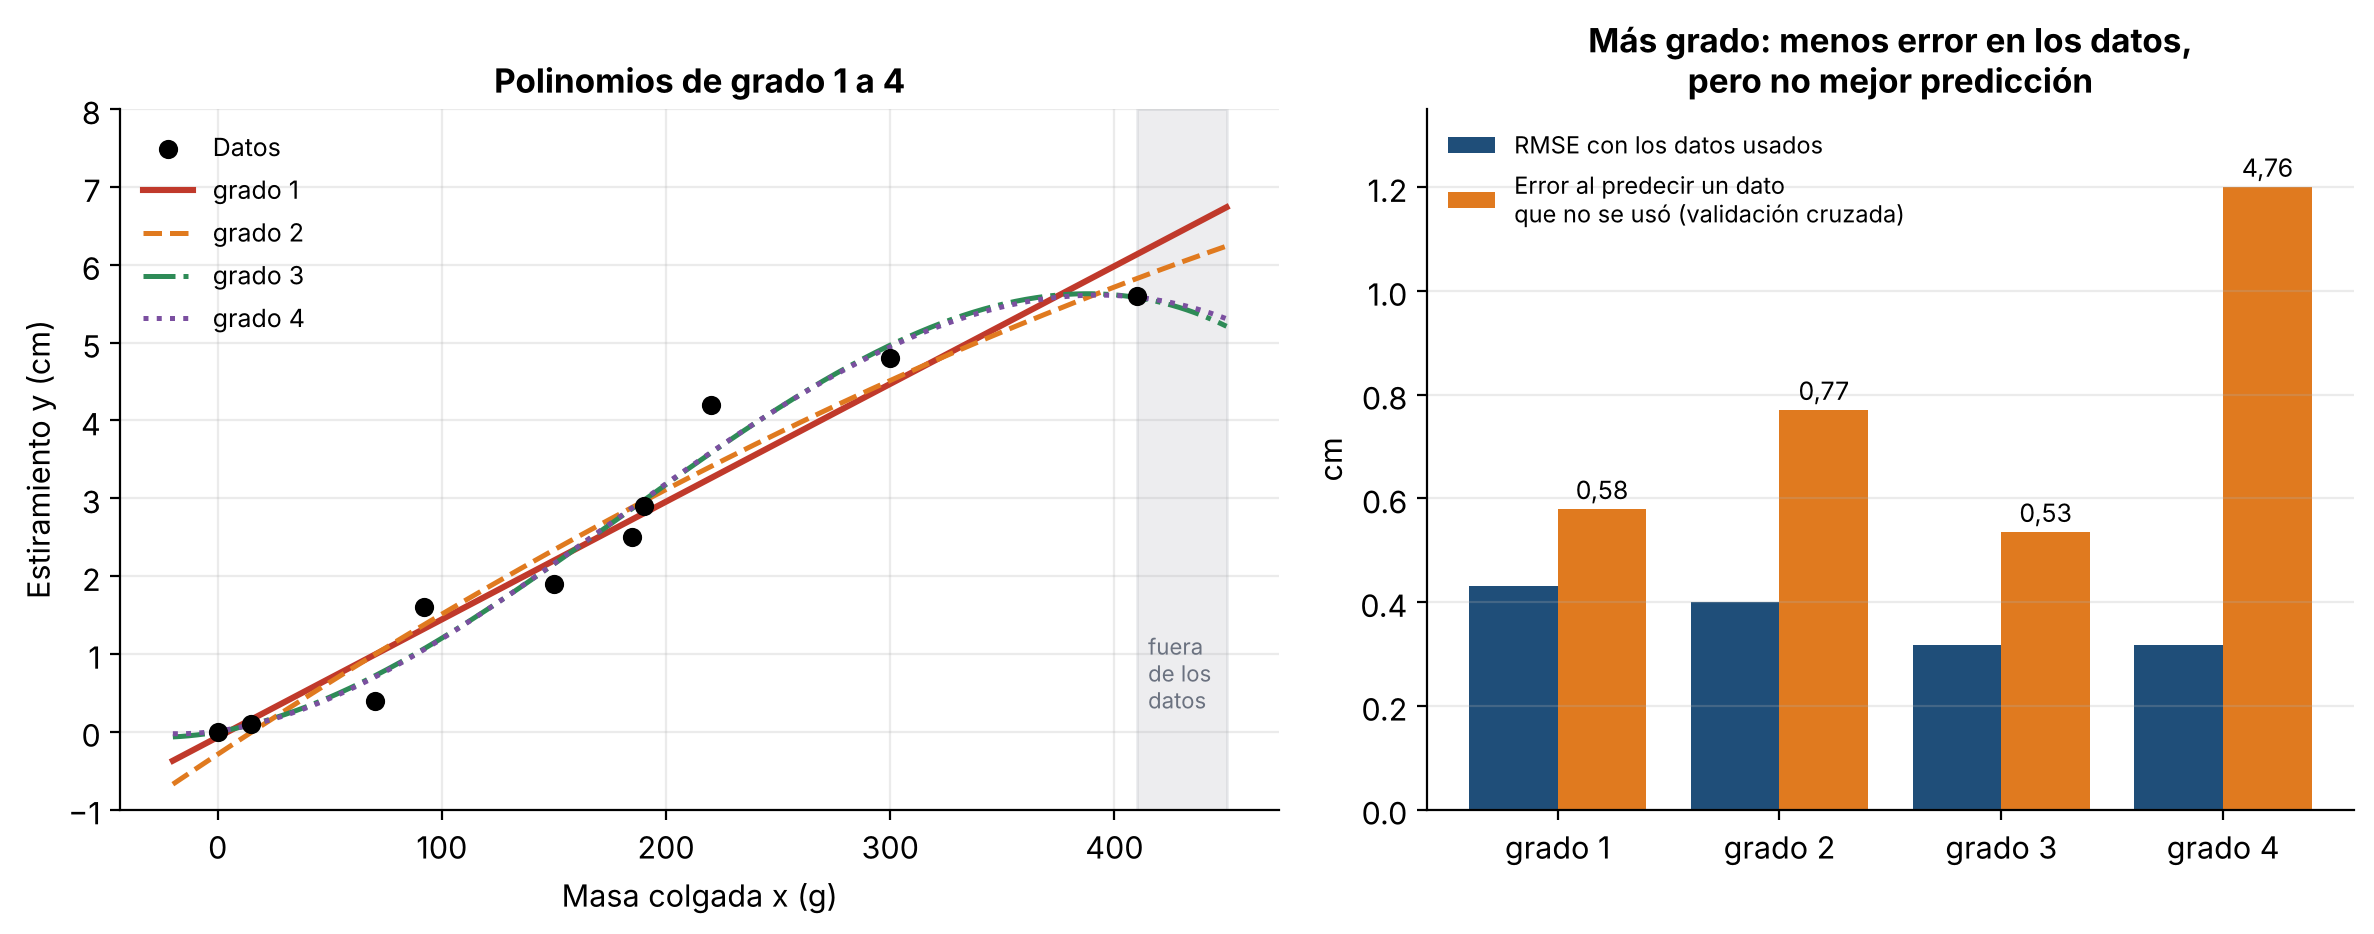
\includegraphics[width=0.92\linewidth]{15_polinomios.png}\par\vspace{0.2em}
  {\small Un polinomio de mayor grado \textbf{siempre} reduce $S$ (tiene más parámetros), pero eso no significa que
  describa mejor el fenómeno: el de grado 4 se equivoca \vpDcv\ cm al predecir un dato que no usó.}
\end{frame}

\begin{frame}{11.7 Comparación de modelos}
  \centering\footnotesize
  \resizebox{\linewidth}{!}{%
  \begin{tabular}{lcccccc}
    \toprule
    Modelo & $S$ (cm$^2$) & RMSE (cm) & $R^2$ & $R^2$ ajust. & Error al predecir & $t$ del término nuevo \\
    \midrule
    \rowcolor{azulclaro}
    Lineal (Hooke) & \vpAS & \vpArmse & \vpArr & \vpAra & \vpAcv & $\vpAt>\vpAtc$ \ \textcolor{verde}{\checkmark} \\
    Grado 2 & \vpBS & \vpBrmse & \vpBrr & \vpBra & \vpBcv & $\vpBt<\vpBtc$ \ \textcolor{rojo}{$\times$} \\
    Grado 3 & \vpCS & \vpCrmse & \vpCrr & \vpCra & \vpCcv & $\vpCt<\vpCtc$ \ \textcolor{rojo}{$\times$} \\
    Grado 4 & \vpDS & \vpDrmse & \vpDrr & \vpDra & \vpDcv & $\vpDt<\vpDtc$ \ \textcolor{rojo}{$\times$} \\
    \midrule
    $y=ax$ (por el origen) & \vorS & \vorRmse & \multicolumn{4}{l}{$a=\vorA$ cm/g, \ $k=\vorK$ N/m} \\
    \bottomrule
  \end{tabular}}
  \vspace{0.5em}
  \begin{columns}[T]
    \column{0.49\textwidth}\footnotesize
    \textbf{$t$ del término nuevo:} si $|t|$ no supera el valor crítico, ese coeficiente podría ser 0.
    \textbf{Prueba F} (¿la mejora sobre la recta es real?): $F_2=\vpBF<\vpBFc$, \ $F_3=\vpCF<\vpCFc$,
    \ $F_4=\vpDF<\vpDFc$. Ninguna mejora es significativa al 95\,\%.
    \column{0.49\textwidth}
    \begin{resultado}[fontupper=\footnotesize]
      La curvatura no es significativa con estos datos: \textbf{la recta es el modelo adecuado} y forzarla por el
      origen casi no cambia $S$ (Hooke puro).
    \end{resultado}
  \end{columns}
\end{frame}

% =====================================================================
\section{Influencia de un dato (opción B)}

\begin{frame}{12. Análisis adicional: influencia de un dato}
  \begin{columns}[c]
    \column{0.58\textwidth}
    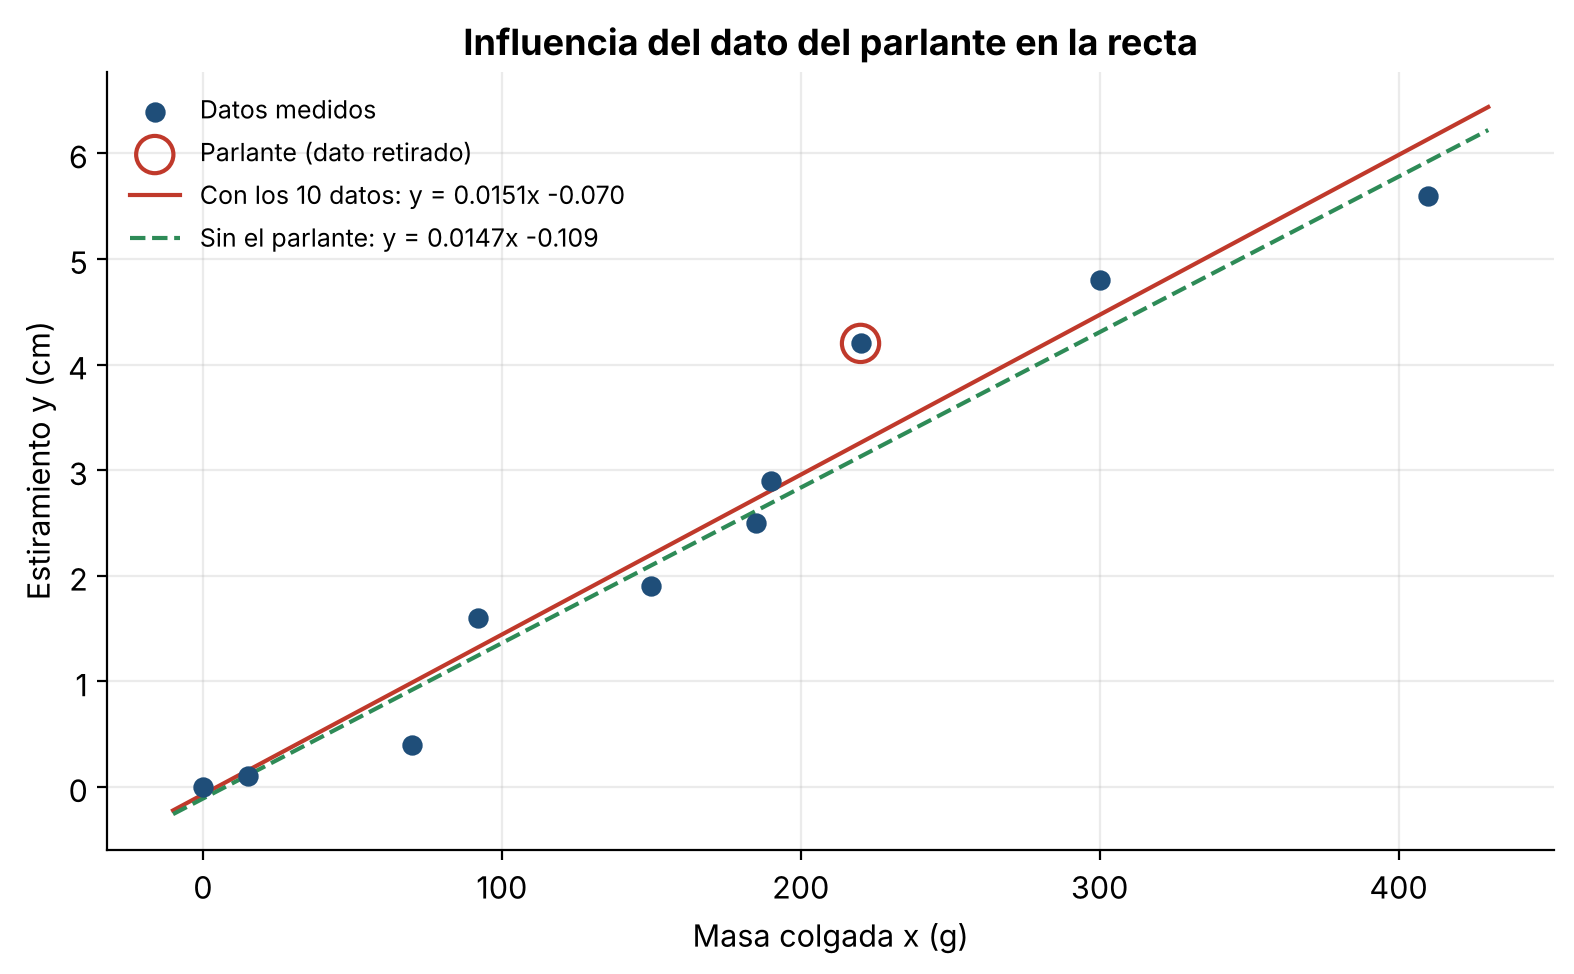
\includegraphics[width=\linewidth]{08_influencia.png}
    \column{0.4\textwidth}
    \centering\small
    \begin{tabular}{lrr}
      \toprule
      & 10 datos & Sin parlante \\
      \midrule
      $a$ (cm/g) & 0,01514 & 0,01472 \\
      $b$ (cm) & $-0{,}070$ & $-0{,}109$ \\
      $S_{\min}$ (cm$^2$) & 1,86 & 0,86 \\
      RMSE (cm) & 0,43 & 0,31 \\
      $R^2$ & 0,9474 & 0,9731 \\
      $k$ (N/m) & 64,7 & 66,6 \\
      \bottomrule
    \end{tabular}
  \end{columns}
  \vspace{0.3em}
  \begin{resultado}[fontupper=\small]
    La pendiente cambia $-2{,}7$\,\% y el nuevo $k$ queda dentro del intervalo de confianza. El parlante es un dato
    \textbf{atípico pero poco influyente}: su masa está cerca del centro de los datos.
  \end{resultado}
\end{frame}

% =====================================================================
\section{Constante del resorte}

\begin{frame}{13. Interpretación física: constante del resorte}
  La pendiente relaciona estiramiento y masa: $a^*=g/k$. En unidades del SI:
  \[ a^*=0{,}0151353\ \frac{\text{cm}}{\text{g}}=0{,}151353\ \frac{\text{m}}{\text{kg}}
     \quad\Rightarrow\quad k=\frac{g}{a^*}=\frac{9{,}8\ \text{m/s}^2}{0{,}151353\ \text{m/kg}}\approx 64{,}7\ \text{N/m}. \]
  \begin{resultado}
    \centering $k=\vkVal\pm\vuK$ N/m \qquad (intervalo de confianza 95\,\%: \vkLo\ a \vkHi\ N/m)
  \end{resultado}
  \small
  Hacen falta unos 64,7 N (el peso de unos 6,6 kg) para estirar este resorte un metro. De forma práctica: cada
  100 g colgados lo estiran aproximadamente 1,5 cm.
\end{frame}

% =====================================================================
\section{Conclusiones y limitaciones}

\begin{frame}{14. Conclusiones (1/2)}
  \small
  \begin{enumerate}
    \item \textbf{Respuesta a la pregunta central.} El Cálculo Multivariable convierte ``hallar la mejor recta''
          en minimizar $S(a,b)$: las derivadas parciales y $\nabla S=0$ dan la recta; el Hessiano demuestra que
          es un mínimo; la superficie, las secciones y las curvas de nivel permiten verlo.
    \item \textbf{Resultado.} La mejor recta es $y=0{,}0151x-0{,}070$ (cm, con $x$ en g), con $S=1{,}86$ cm$^2$.
    \item \textbf{El mínimo es único.} $\det H>0$ y $S_{aa}>0$; como $H$ es constante, $S$ es convexa.
    \item \textbf{Los tres métodos coinciden.} A mano, código propio y \texttt{numpy.polyfit} dan los mismos
          parámetros; el computador verificó el resultado, no lo reemplazó.
  \end{enumerate}
\end{frame}

\begin{frame}{14. Conclusiones (2/2)}
  \small
  \begin{enumerate}\setcounter{enumi}{4}
    \item \textbf{La Ley de Hooke se cumple razonablemente.} $R^2=0{,}9474$, intercepto compatible con cero y
          residuos sin patrón. \textbf{$k=\vkVal\pm\vuK$ N/m} (entre \vkLo\ y \vkHi\ N/m al 95\,\%).
    \item \textbf{Ninguna otra función es mejor.} Los polinomios de grado 2 a 4 bajan $S$, pero sus términos
          extra no son significativos y predicen peor datos nuevos.
    \item \textbf{El error no viene de los instrumentos.} El RMSE (\vrmseMm\ mm $\approx$ \vrmseG\ g) es unas
          \vrazon\ veces la incertidumbre de la regla; la gramera es despreciable. Domina el método de medición.
    \item \textbf{Las curvas de nivel enseñan algo que la recta no muestra:} pendiente e intercepto se
          compensan.
    \item \textbf{Un dato atípico no siempre es influyente:} sin el parlante, $S$ baja a menos de la mitad, pero
          $k$ cambia menos del 3\,\%; el dato más influyente es el alicate.
  \end{enumerate}
\end{frame}

\begin{frame}{14.1 Reflexión crítica y limitaciones}
  \small
  \begin{itemize}
    \item \textbf{Pocos datos.} Con 10 puntos la curvatura leve no se distingue del ruido (prueba F no
          significativa) y el intervalo de $k$ es amplio (\vkRango\ N/m).
    \item \textbf{Una sola lectura por objeto.} Sin repeticiones no se estima la dispersión de cada punto; solo
          se pudo usar la incertidumbre tipo B de los instrumentos.
    \item \textbf{Método indirecto.} El estiramiento sale de restar tres lecturas; los objetos tienen formas
          distintas y no cuelgan del mismo punto. Por eso el RMSE (0,43 cm) supera el error instrumental (0,05 cm).
    \item \textbf{Tensión inicial.} Con cargas livianas el resorte casi no se estira.
    \item \textbf{Rango de validez.} La recta solo vale entre 0 y 410 g: no se debe extrapolar.
    \item \textbf{Registro fotográfico incompleto.} Cuatro cargas tienen imágenes ilustrativas.
  \end{itemize}
\end{frame}

\begin{frame}{14.2 Recomendaciones para un próximo experimento}
  \begin{columns}[T]
    \column{0.49\textwidth}
    \begin{block}{Medición}
      \begin{itemize}\small
        \item Usar pesas de masa conocida con un mismo gancho.
        \item Medir directamente la posición del extremo inferior del resorte (una sola lectura en vez de tres).
        \item Repetir cada lectura tres veces para poner barras de error tipo A.
      \end{itemize}
    \end{block}
    \column{0.49\textwidth}
    \begin{block}{Diseño}
      \begin{itemize}\small
        \item Agregar masas entre 0 y 100 g para estudiar la tensión inicial.
        \item Más datos en los extremos para estrechar el intervalo de $k$.
        \item Fotografiar todas las cargas.
      \end{itemize}
    \end{block}
  \end{columns}
\end{frame}

\begin{frame}{Referencias}
  \small
  \begin{itemize}
    \item Harris, C. R., Millman, K. J., van der Walt, S. J., et al. (2020). Array programming with NumPy.
          \emph{Nature}, 585, 357--362.
    \item Hunter, J. D. (2007). Matplotlib: A 2D graphics environment. \emph{Computing in Science \&
          Engineering}, 9(3), 90--95.
    \item JCGM (2008). \emph{Evaluación de datos de medición --- Guía para la expresión de la incertidumbre de
          medida (GUM)}. JCGM 100:2008.
    \item Montgomery, D. C., Peck, E. A. y Vining, G. G. (2012). \emph{Introduction to Linear Regression
          Analysis} (5.ª ed.). Wiley.
    \item Molina, A. (2026). \emph{Proyecto de Cálculo Multivariable: Regresión lineal y optimización mediante
          funciones de varias variables}. Universidad Cooperativa de Colombia.
  \end{itemize}
\end{frame}

{\setbeamercolor{background canvas}{bg=azul}
\begin{frame}[plain]
  \centering
  {\color{white}\Huge\bfseries Gracias}\\[1em]
  {\color{naranja}\Large ¿Preguntas?}\\[2em]
  {\color{white!80}\small $y=0{,}0151\,x-0{,}070$ \quad·\quad $k=\vkVal\pm\vuK$ N/m \quad·\quad $R^2=0{,}947$}
\end{frame}}

% =====================================================================
\appendix

\begin{frame}{Apéndice A. Diagramas de flujo: sumas y calidad}
  \centering
  \begin{columns}[c]
    \column{0.48\textwidth}\centering
    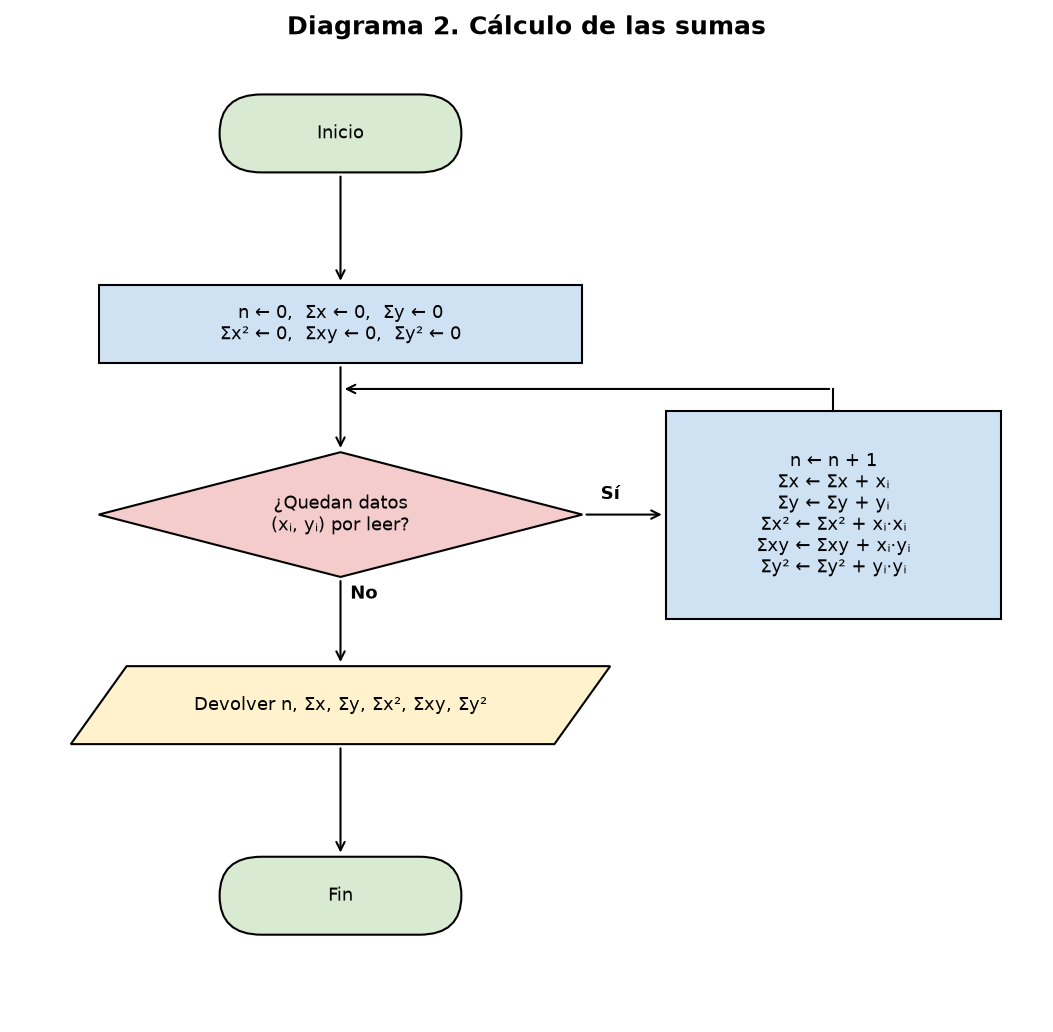
\includegraphics[height=0.72\textheight]{diagrama_2_sumas.png}\\{\scriptsize Diagrama 2: cálculo de las sumas}
    \column{0.48\textwidth}\centering
    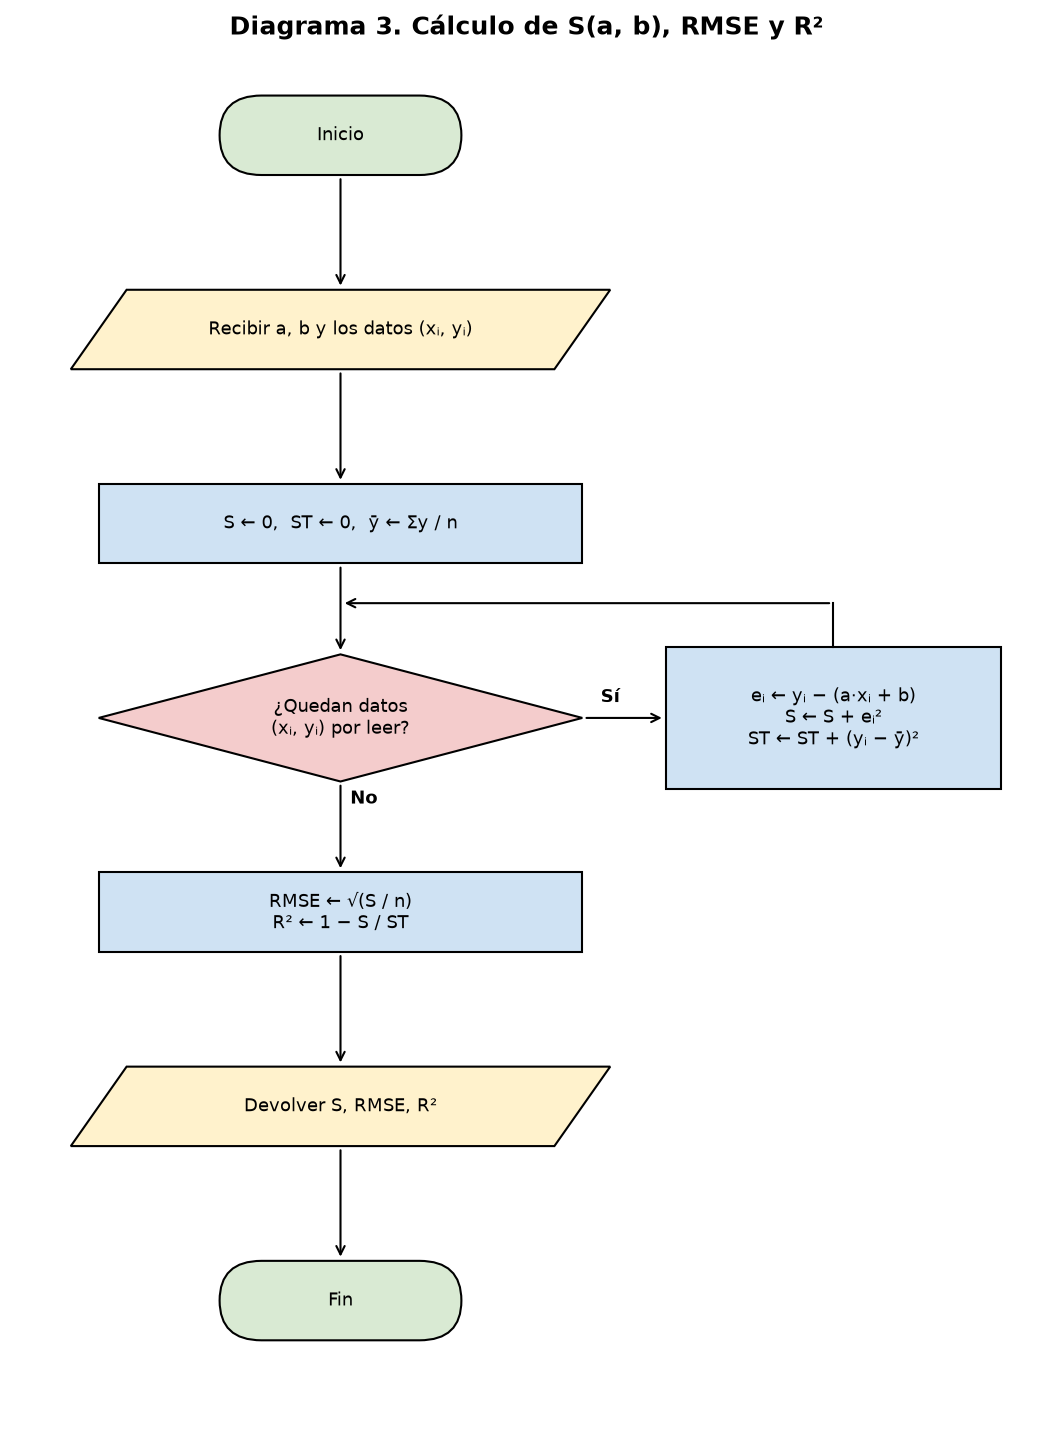
\includegraphics[height=0.72\textheight]{diagrama_3_error.png}\\{\scriptsize Diagrama 3: $S$, RMSE y $R^2$}
  \end{columns}
\end{frame}

\begin{frame}{Apéndice B. Valores predichos y residuos}
  \centering\small
  \begin{tabular}{lrrrr}
    \toprule
    Objeto & $x$ (g) & $y$ medido (cm) & $\hat y$ predicho (cm) & Residuo $e$ (cm) \\
    \midrule
    Resorte sin carga & 0 & 0,0 & $-0{,}07$ & $+0{,}07$ \\
    Llave grande & 15 & 0,1 & 0,16 & $-0{,}06$ \\
    Tornillo grande & 70 & 0,4 & 0,99 & $-0{,}59$ \\
    Taza plástica & 92 & 1,6 & 1,32 & $+0{,}28$ \\
    Rollo de cinta & 150 & 1,9 & 2,20 & $-0{,}30$ \\
    Herradura & 185 & 2,5 & 2,73 & $-0{,}23$ \\
    Teléfono LG & 190 & 2,9 & 2,81 & $+0{,}09$ \\
    \rowcolor{naranja!12}
    Reproductor / parlante & 220 & 4,2 & 3,26 & $+0{,}94$ \\
    Libro pequeño & 300 & 4,8 & 4,47 & $+0{,}33$ \\
    Alicate & 410 & 5,6 & 6,14 & $-0{,}54$ \\
    \bottomrule
  \end{tabular}
\end{frame}

\begin{frame}{Apéndice C. Desarrollo del Hessiano y de los valores propios}
  Valores propios: $\lambda^2-825\,848\,\lambda+5\,862\,864=0$ \ (traza $=825\,848$).
  \[ \lambda_{1,2}=\frac{825\,848\pm 825\,833{,}801}{2}\quad\Rightarrow\quad \lambda_1=825\,840{,}9,\qquad \lambda_2=7{,}099. \]
  Ambos positivos: $H$ es definida positiva.

  \medskip
  Comprobación de las ecuaciones normales con $a^*$ y $b^*$:
  \begin{align*}
    412\,914\,(0{,}0151353)+1632\,(-0{,}0700810)&=6135{,}21\approx 6135{,}2\\
    1632\,(0{,}0151353)+10\,(-0{,}0700810)&=24{,}0000
  \end{align*}
\end{frame}

\begin{frame}{Apéndice D. Fórmulas de incertidumbre usadas}
  \small
  \begin{columns}[T]
    \column{0.49\textwidth}
    \textbf{Tipo B (instrumentos)}, distribución uniforme de ancho igual a la resolución $r$:
    \[ u=\frac{r}{2\sqrt3} \]
    Suma de lecturas independientes: $u_y=\sqrt{u_1^2+u_2^2+u_3^2}$.

    \medskip
    \textbf{Propagación} para $k=g/a$:
    \[ u_k=\left|\frac{\partial k}{\partial a}\right|u_a=\frac{g}{a^2}u_a=k\,\frac{u_a}{a} \]
    \column{0.49\textwidth}
    \textbf{Prueba F} para comparar el polinomio de grado $d$ con la recta:
    \[ F=\frac{(S_1-S_d)/(d-1)}{S_d/(n-d-1)} \]
    \textbf{Validación cruzada} (dejar uno fuera): se ajusta sin el dato $i$, se predice $y_i$ y se promedia el
    error al cuadrado de los $n$ casos.

    \medskip
    \textbf{Monte Carlo:} 20\,000 repeticiones del ajuste perturbando cada lectura dentro de $\pm$ media
    resolución.
  \end{columns}
\end{frame}

\end{document}
